%%%% ijcai22.tex

\typeout{IJCAI--22 Instructions for Authors}

% These are the instructions for authors for IJCAI-22.

\documentclass{article}
\pdfpagewidth=8.5in
\pdfpageheight=11in
% The file ijcai22.sty is NOT the same as previous years'
\usepackage{ijcai22}

% Use the postscript times font!
\usepackage{times}
\usepackage{verbatim} % multiple-line comments 
\usepackage{soul}
\usepackage{url}
\usepackage[hidelinks]{hyperref}
\usepackage[utf8]{inputenc}
\usepackage[small]{caption}
\usepackage{graphicx}
\usepackage{amsmath}
\usepackage{amsthm}
\usepackage{booktabs}
\usepackage{algorithm}
\usepackage{algorithmic}
\usepackage{multirow}
\usepackage{xcolor}

\urlstyle{same}

% the following package is optional:
%\usepackage{latexsym}

% See https://www.overleaf.com/learn/latex/theorems_and_proofs
% for a nice explanation of how to define new theorems, but keep
% in mind that the amsthm package is already included in this
% template and that you must *not* alter the styling.
\newtheorem{example}{Example}
\newtheorem{theorem}{Theorem}

% Following comment is from ijcai97-submit.tex:
% The preparation of these files was supported by Schlumberger Palo Alto
% Research, AT\&T Bell Laboratories, and Morgan Kaufmann Publishers.
% Shirley Jowell, of Morgan Kaufmann Publishers, and Peter F.
% Patel-Schneider, of AT\&T Bell Laboratories collaborated on their
% preparation.

% These instructions can be modified and used in other conferences as long
% as credit to the authors and supporting agencies is retained, this notice
% is not changed, and further modification or reuse is not restricted.
% Neither Shirley Jowell nor Peter F. Patel-Schneider can be listed as
% contacts for providing assistance without their prior permission.

% To use for other conferences, change references to files and the
% conference appropriate and use other authors, contacts, publishers, and
% organizations.
% Also change the deadline and address for returning papers and the length and
% page charge instructions.
% Put where the files are available in the appropriate places.

% PDF Info Is REQUIRED.
% Please **do not** include Title and Author information
\pdfinfo{
/TemplateVersion (IJCAI.2022.0)
}

\title{CS5487 Course Porject -MNIST}

% % Single author syntax
% \author{
%     Author Name
%     \affiliations
%     Affiliation
%     \emails
%     pcchair@ijcai-22.org
% }

% Multiple author syntax (remove the single-author syntax above and the \iffalse ... \fi here)
% Check the ijcai22-multiauthor.tex file for detailed instructions
% \iffalse
\author{
WANG Xuezhen$^1$ 56199738
\and
HUANG Yixiao$^1$ 56237342
% \and
% Third Author$^{2,3}$\And
% Fourth Author$^4$
\affiliations
$^1$City University of Hong Kong
% \\
% $^2$Second Affiliation\\
% $^3$Third Affiliation\\
% $^4$Fourth Affiliation
\emails
\{xuezhwang2-c, yixihuang9-c\}@my.cityu.edu.hk
% ,
% third@other.example.com,
% fourth@example.com
}
% \fi

\begin{document}

\maketitle

% \begin{abstract}
%   The {\it IJCAI--22 Proceedings} will be printed from electronic
%   manuscripts submitted by the authors. The electronic manuscript will
%   also be included in the online version of the proceedings. This paper
%   provides the style instructions.
% \end{abstract}

\section{Introduction}
In this project, we train different machine learning models based on a given MNIST handwritten digit dataset, aiming to explore different algorithms' performance as well as achieve a high classification accuracy.

\paragraph{Background.}
In the field of computation vision, the Modified National Institute of Standards and Technology (MNIST) is the standard dataset \cite{deng2012mnist}. This famous dataset, which consists of a collection of handwritten digit pictures, has been utilized widely in machine learning and optical character recognition research since its publication in 1999. In the real world, digit recognition systems can significantly reduce human effort and accurately recognize digits from various resources such as bank cheques, mails, and drafts, as well as in a variety of demanding scenarios such as numeric entries in tax forms, processing bank cheque amounts, and recognizing vehicle number plates, among others.

\section{Road Map}
See Figure~\ref{fig:map} in Appendix~\ref{map}.

\section{Methodology}
\subsection{Data Augmentation and Normalization}
Data augmentation is the process of making simple and complex changes to data, such as flipping or style transfer, in order to expand the data size to match the dimensionality requirement. We'll use several simple but effective techniques to "perturb" the original photos in order to obtain more data, such as \textbf{rotating, zooming, and translating}. Moreover, we perform a grayscale normalization to reduce the effect of illumination’s differences. 
\subsection{Feature Extraction} \label{feature}
Techniques for extracting features are useful in a variety of image processing applications. As features describe an image's behavior, they reveal its position in terms of storage required, classification efficiency, and, of course, time consumption. We consider three methods of feature extractions in this project:
\begin{enumerate}
    \item We use all images' pixel values to form a feature vector.
    \item We form a window of size $2\times2$ centered around pixels and extract the \textbf{average values} of the $4$ pixels to be its feature value. Notice that this method implicitly reduces the number of features for each instance.
    \item We consider the \textbf{edge information} of images. Specifically, we first apply an edge-finding filter on each image and then use all pixel values of each transformed image to form a feature vector. We rely on the third party code \emph{Python Imaging Library} for implementation \cite{PIL}.
\end{enumerate}
\subsection{Dimensionality Reduction}
The transfer of data from a high-dimensional space to a low-dimensional space so that the low-dimensional representation preserves some significant aspects of the original data, ideally near to its inherent dimension, is known as dimensionality reduction. Working with high-dimensional spaces can be inconvenient for a variety of reasons: raw data is generally sparse as a result of dimensionality's curse, and data analysis is usually computationally intractable. In this project, we will consider to apply three dimensionality reduction technics to the dataset, specifically: \textbf{Principle Component Analysis (PCA), Kernel Principle Component Analysis (KPCA), and Linear Discriminant Analysis (LDA)}.
PCA conducts a linear mapping of data from a higher-dimensional space to a lower-dimensional space with the goal of maximizing the data's variance in the low-dimensional representation. KPCA is a PCA modification that uses the kernel approach to use in non-linear situations. It has the ability to create nonlinear mappings that optimize data variance. However, both of them does not utilize the label information of the training dataset. Hence, when the noise variance is larger than the signal variance, it will result a extremely bad performance. LDA is used to determine a linear combination of features that distinguishes two or more groups of classes. It makes an explicit attempt to represent the differences between the data classes. However, It can only handles linear projection and its maximum number of components is constrained to be $C-1$ where $C$ is the number of classes. In our project, implementation relies on the third party library \emph{Scikit-learn} \cite{pedregosa2011scikit}.

\subsection{Logistic Regression}
The probability for classification issues with two possible outcomes are modelled using logistic regression. It employs the logistic function to compress the output of a linear equation between $0$ and $1$ instead of fitting a straight line or hyperplane. It requires less computational power to train the model as its number of parameters is linearly related to the feature dimension. However, it can only perfectly classify problems with linear decision boundary. In our project, implementation relies on the third party library \emph{Scikit-learn} \cite{pedregosa2011scikit}. \cite{pedregosa2011scikit}.

\subsection{Naive Bayes Classifier}
Naive Bayes Classifier is a classification method based on Bayes Theorem and the assumption of predictor independence. In basic words, it posits that the existence of one feature in a class is independent to the presence of any other feature. The advantage is that if the model assumption is true, the probability distribution of class is the best we can do. However, since we only need to classify the data instead of generating the distribution, generative model requires an additional middle man which may induce error and much more data to train the parameters. In our project, implementation relies on the third party library \emph{Scikit-learn} \cite{pedregosa2011scikit}.

\subsection{Support Vector Machine}
Support Vector Machine is effective in high dimensional spaces and also memory efficient as the fact that it relies on only those support vectors, though on the other hand it is inefficient for large dataset. In this project, we will consider the \textbf{linear SVM} and apply the \textbf{kernel trick} such that it can learn a non-linear decision boundary. In our project, implementation relies on the third party library \cite{pedregosa2011scikit}.

\emph{Remark: Throughout the project we will use SVM to denote linear SVM, and kSVM to denote the SVM using the kernel trick}
\emph{Scikit-learn}.

\subsection{Neural Network} \label{nn}
Recently, deep learning algorithms have been one of the most popular models adopted in pattern recognition tasks. The capability of learning complex and non-linear correlations from a large number of examples makes multi-layer networks an ideal candidate for image recognition problems \cite{Lecun1998}. In our project, we used two different neural network architectures, which are simple neural networks with four layers (MLP) and convolutional neural network (CNN). The disadvantage of the simple neural network or multi-layer perceptron is that the topology of the input is not utilized in training as we need to flatten the 2-D image to 1-D input. However, images have a strong 2-D local correlations and spatiality, which are then ignored in the networks. In comparison, CNN is famous in extracting local features via the convolutional layers as it forces the receptive fields of hidden units to be local \cite{Lecun1998}. 
\begin{comment}
Self-attention-based networks have been popular in naturla language processing and image classification. In particular Vision Transformer has outperformed CNN in image classification tasks. However, the high performance of ViT requires an intensive pre-training use a large-size datasets. It's stated that when equipped with some special modules, Shifted Patch Tokenization (SPT) and Locality Self-Attention (LSA), ViT is also able to perform well in small-size datasets. In our project, we are curious to find out whether this architecture will also be helpful in our task \cite{ViTsmall}.
\end{comment}
\subsubsection{Convolutional Neural Network}
CNN  has three main types of layers, which are:
\begin{itemize}
    \item Convolutional Layer
    \item Pooling Layer
    \item Fully-connected Layer
\end{itemize}

\textbf{Convolutional Layer. }
The main component of Convolutional Layer is the feature extractor, which are also known as a kernel or filter. As illustrated in Figure ~\ref{CL}, the filter convolves with the image and create a feature map. Specifically, the module calculates the dot product between the filter and an area of the image. Then the filter slides across the image and repeat the operation until the kernel has gone through the entire image. Notably, each value in the feature map is only correlated with part of the image, which is called the receptive field. Thus it emphasizes the local connectivity compared with the fully connected layers\cite{ibmconv}. Typically, the filter size is a $3 \times 3$, $5 \times 5$ or $7 \times 7$ matrix. \textbf{We tried these three options in our experiments.}

\begin{figure}[h]
    \centering
    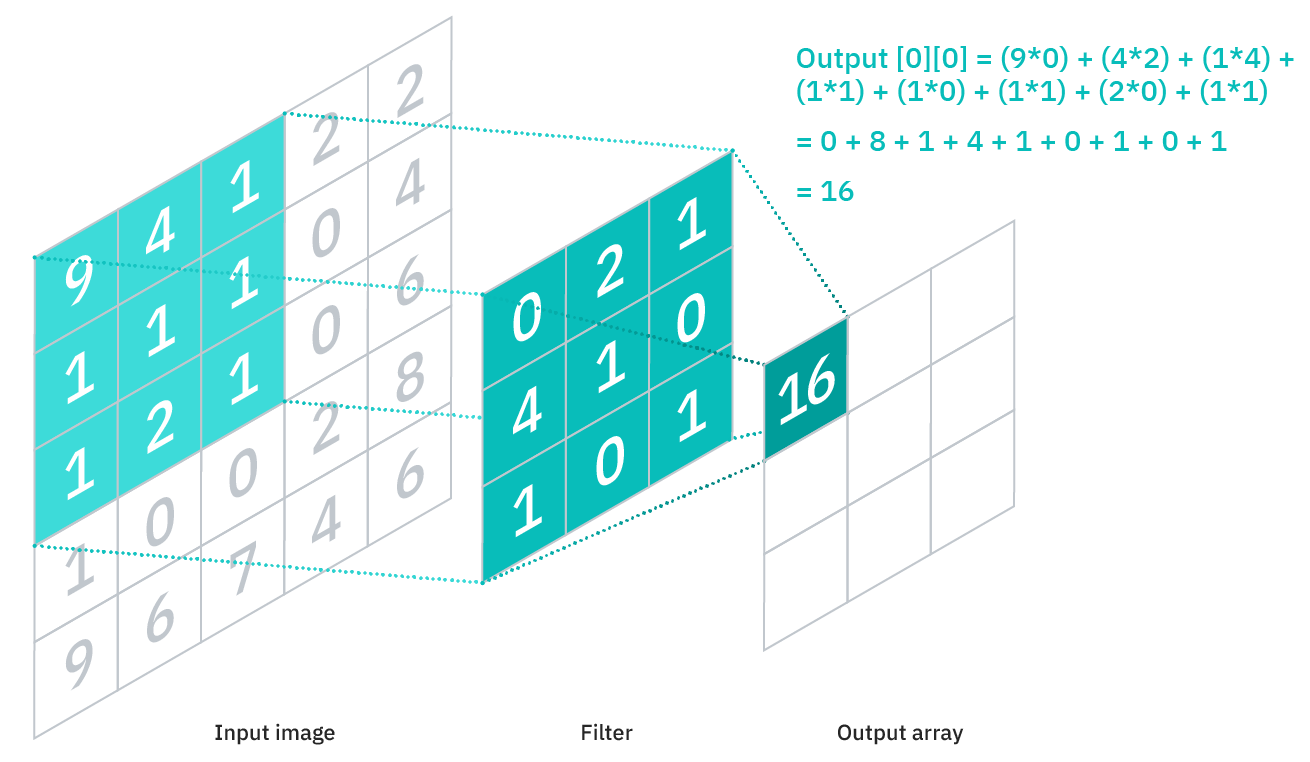
\includegraphics[width=0.5\textwidth]{figure/Convolve.png}
    \caption{Convolutional Layer}
    \label{CL}
\end{figure}
\textbf{Pooling Layer. }
Pooling layer is used to reduce the dimension of the feature map. It also use a filter to move across the input and apply an aggregation function to the values in the feature map. There are two popular aggregation functions which are: 
\begin{itemize}
    \item {Max Pooling}: Select the pixel with the maximum value to the output.
    \item {Average Pooling}: Calculate the average value across the receptive field to the output.
\end{itemize}
Pooling layer is beneficial in reducing number of parameters and limiting the risk of overfitting \cite{ibmconv}.
\\ \\ 
\textbf{Fully-connected Layer}
As indicated by its name, in fully-connected layer, each neuron in the output layer is connected to a node in the previous layer. We also use one fully-connected layer with softmax activation function to render the probability that the input represents each digit.

\section{Experiments Setup and Evaluation}
\subsection{Data}
The dataset used contains $4000$ images and each example has the dimension of $28 \times 28$ which has been flattened to a vector of size $1 \times 784$. We will run two independent trials on the data where each trial splits the images evenly as training set and test set based on the given index (i.e., each with $2000$ images).
\subsection{Data Pre-processing} \label{aug}
\subsubsection{Data Augmentation and Normalization}
\textbf{Data Augmentation. } For traditional machine learning algorithms, to generate more samples from the training set with $n=2000$ data points, we first augment it to a dataset with $n' = 8000$. $2000$ of them are translated by $1$ pixel randomly along all possible directions, another $2000$ are rotated randomly in a range of angles in $[0, 20]$ degree, the final $2000$ are randomly scaled by a factor in $[0.7, 1]$. Notably, for CNN network, we adopted a \textbf{different augmentation strategy} to transform the original dataset instead of generating new data. We used function \emph{ImageDataGenerator} from the third party library \emph{Tensorflow} \cite{tensorflow2015-whitepaper}. We found using this strategy will lead to a better performance on the test set and challenge test, which will be discussed in the analysis of CNN in Section ~\ref{aug_survey}. For the augmentation setting, we construct an augmentation layer containing four operations:
\begin{itemize}
    \item{Randomly rotate some training images by 20 degrees}
    \item{Randomly Zoom from 70\% (zoom in) to 130\% (zoom out). }
    \item{Randomly shift images horizontally by 10\% of the width}
    \item{Randomly shift images vertically by 10\% of the height}
\end{itemize}
\textbf{Normalization.} Normalization is simply to transform the features from \textbf{[0, 255] to [0, 1]} such that most of the algorithms may converge faster.
\subsubsection{Feature Extraction}
See above Section~\ref{feature} for a detailed explanation.
\subsubsection{Dimensionality Reduction}
\paragraph{PCA and kPCA.}
The Feature Extraction will produce three kinds of dataset. We need to select the number of components in PCA and kPCA (with $4^{th}$ order polynomial kernel) for each of them. To do that, we plot the variance kept/explained values againt the number of components to select the minimum number of components which we can reserve enough variance of data/explained values.

\begin{figure}[!htb]
\minipage{0.24\textwidth}
  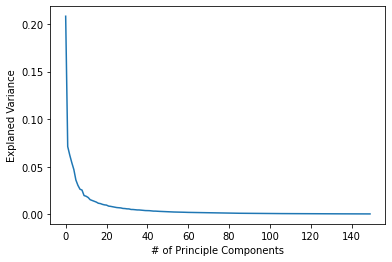
\includegraphics[width=\linewidth]{figure/pca_none.png}
%   \caption{PCA}\label{fig:pca_none}
\endminipage\hfill
\minipage{0.24\textwidth}
  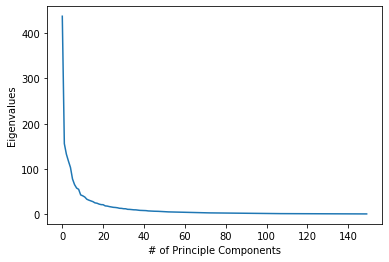
\includegraphics[width=\linewidth]{figure/kpca_none.png}
%   \caption{kPCA}\label{fig:kpca_none}
\endminipage
\caption{Feature Extraction 1: PCA and kPCA}
\label{feature1}
\end{figure}


From the Figure~\ref{feature1}, in terms of the data generated from the first feature extraction, we observe that \textbf{40} principle components for both PCA and kPCA (with $4^{th}$ order polynomial kernel) are enough to maintain sufficient variance of data/explained values.

\begin{figure}[!htb]
\minipage{0.24\textwidth}
  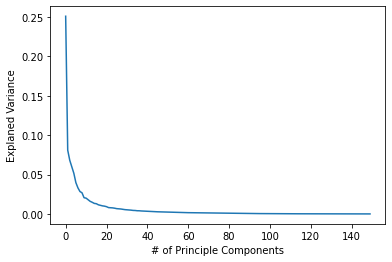
\includegraphics[width=\linewidth]{figure/pca_avg.png}
%   \caption{PCA}\label{fig:pca_none}
\endminipage\hfill
\minipage{0.24\textwidth}
  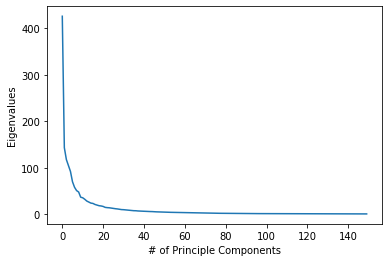
\includegraphics[width=\linewidth]{figure/kpca_avg.png}
%   \caption{kPCA}\label{fig:kpca_none}
\endminipage
\caption{Feature Extraction 2 (Average): PCA and kPCA}
\label{feature2}
\end{figure}

We may observe that Figure~\ref{feature2} is very similar to Figure~\ref{feature1} which is very interesting. By choosing the second method of feature extracting, we compress the $28\times 28$ image into a $7 \times 7$ one which significantly reduce the number of features, however, the number of features required in order to maintain a valid variable variance/explained values are still very much the same. Hence, we still adopt \textbf{40} principle components for both PCA and kPCA

\begin{figure}[!htb]
\minipage{0.24\textwidth}
  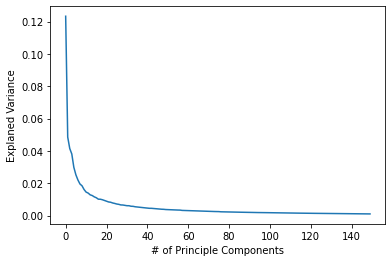
\includegraphics[width=\linewidth]{figure/pca_edge.png}
%   \caption{PCA}\label{fig:pca_none}
\endminipage\hfill
\minipage{0.24\textwidth}
  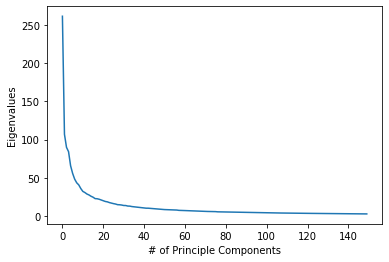
\includegraphics[width=\linewidth]{figure/kpca_edge.png}
%   \caption{kPCA}\label{fig:kpca_none}
\endminipage
\caption{Feature Extraction 3 (Edge): PCA and kPCA}
\label{feature3}
\end{figure}

Finally, we observe that (though not that obvious) the curve Figure~\ref{feature3} decreases slower than above $2$ feature extraction methods. Hence, in order to maintain a a valid variable variance/explained values, we keep \textbf{60} principle components for both PCA and kPCA.

\paragraph{LDA.}
Regarding the LDA, since the maximum number of features it can keep is $C-1 = 9$ for our project. Since the original number of features are either $784$ for feature extraction methods $1$ and $3$, or $196$ for feature extraction methods $2$ which is much larger than $9$. We will use the largest number of dimensions LDA can keep, i.e. \textbf{9}.

\subsection{Algorithms}
\subsubsection{Logistic Regression}

\emph{Remark: As there are in total 3 (number of methods of feature selections) $\times$ 4 (w/o, w/ 3 kinds of dimensionality reduction) $\times$ 2 (trials) = 24 possible combinations which are impossible to put all the figures within one report. For each parts where we insert figures, it use 4 figures, specifically, the figures under the condition w/o, w/ 3 kinds of dimensionality reduction when we use the first trial training data and the first feature extraction method to demonstrate the idea.}

\paragraph{Hyper-Parameter Tuning.}

We use the regularized logistic regression which in the \emph{Scikit-Learn package} has an hyper-parameter $C$, i.e., inverse of regularization strength and we need to find the best $C$ for the model.
\begin{figure}[!htb]
\minipage{0.24\textwidth}
  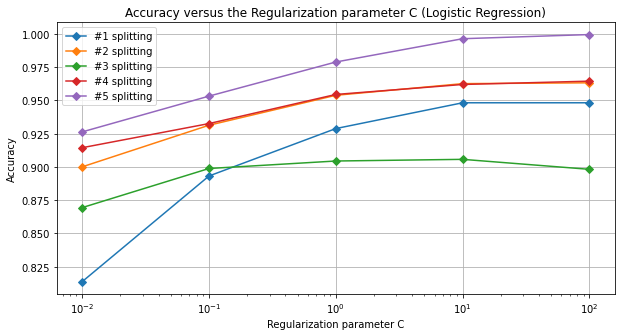
\includegraphics[width=\linewidth]{figure/logit.png}
%   \caption{PCA}\label{fig:pca_none}
\endminipage\hfill
\minipage{0.24\textwidth}
  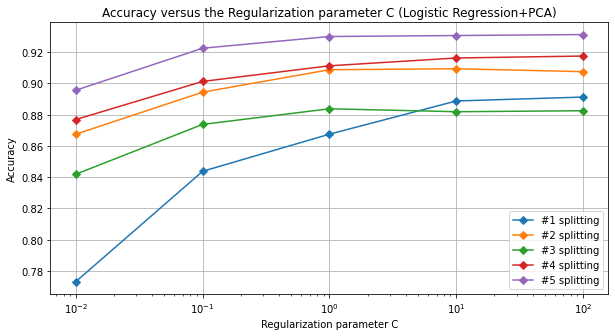
\includegraphics[width=\linewidth]{figure/logit_pca.png}
%   \caption{kPCA}\label{fig:kpca_none}
\endminipage\hfill
\minipage{0.24\textwidth}
  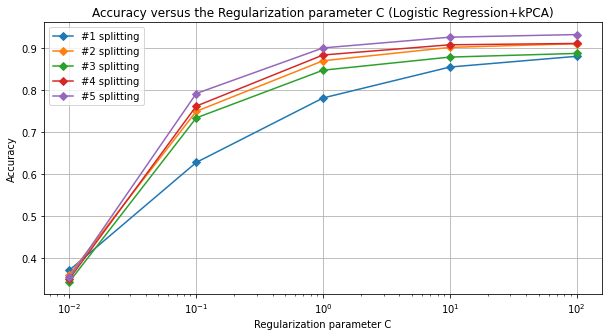
\includegraphics[width=\linewidth]{figure/logit_kpca.png}
%   \caption{PCA}\label{fig:pca_none}
\endminipage\hfill
\minipage{0.24\textwidth}
  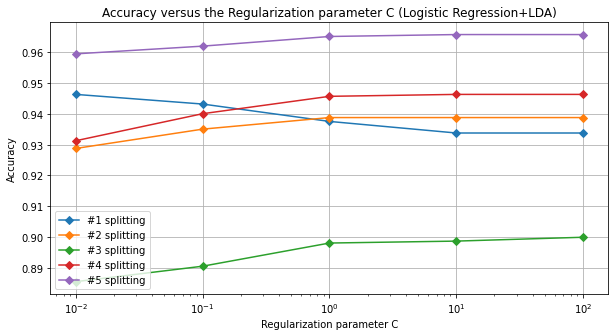
\includegraphics[width=\linewidth]{figure/logit_lda.png}
%   \caption{kPCA}\label{fig:kpca_none}
\endminipage
\caption{Logistic Regression hyper-parameter tuning for w/o dimensionality reduction, PCA, kPCA, LDA under (trial 1, feature extraction method 1)}
\label{logit_hyper}
\end{figure}

As we observe from Figure~\ref{logit_hyper}, the accuracy score on the cross-validation tends to increase as we increase the value of $C$. When the accuracy does not increase too much as $C$ increases, it indicates a higher chance of overfitting. Hence, for this particular case, we adopt $C = 10, 1, 1, 1$ for  w/o dimensionality reduction, PCA, kPCA, LDA, respectively. We adopt similar methods for other combination of trail and feature extraction methods.

\paragraph{Results.}
We use two metrics to evaluate the result. Specifically, the accuracy rate and the confusion matrix where the latter can also provides us with the information about which two classes are easily to be misclassified.

\begin{table}[!htb]
\begin{tabular}{|c|c|ccc|}
\hline
\textit{\textbf{Algorithm}}                                                                    & \textit{\textbf{Num}}     & \multicolumn{3}{r|}{\textit{\textbf{Feature Extraction Method}}}                                                        \\ \hline
\textit{\textbf{Logistic Reg}}                                                                             & \textit{\textbf{}}        & \multicolumn{1}{c|}{\textit{\textbf{1}}}     & \multicolumn{1}{c|}{\textit{\textbf{2}}}      & \textit{\textbf{3}}      \\ \hline
\multirow{3}{*}{\textit{\textbf{\begin{tabular}[c]{@{}c@{}}w/o dim\\ Reduction\end{tabular}}}} & \textit{\textbf{trial 1}} & \multicolumn{1}{c|}{\textit{\textbf{0.878}}} & \multicolumn{1}{c|}{\textit{\textbf{0.89}}}   & \textit{\textbf{0.856}}  \\ \cline{2-5} 
                                                                                               & \textit{\textbf{trial 2}} & \multicolumn{1}{c|}{\textit{\textbf{0.868}}} & \multicolumn{1}{c|}{\textit{\textbf{0.875}}}  & \textit{\textbf{0.837}}  \\ \cline{2-5} 
                                                                                               & \textit{\textbf{average}} & \multicolumn{1}{c|}{\textit{\textbf{0.873}}} & \multicolumn{1}{c|}{\textit{\textbf{\color{red}0.8825}}} & \textit{\textbf{0.8465}} \\ \hline
\textit{\textbf{}}                                                                             & \textit{\textbf{trial 1}} & \multicolumn{1}{c|}{\textit{\textbf{0.876}}} & \multicolumn{1}{c|}{\textit{\textbf{0.879}}}  & \textit{\textbf{0.863}}  \\ \cline{2-5} 
\textit{\textbf{with PCA}}                                                                     & \textit{\textbf{trial 2}} & \multicolumn{1}{c|}{\textit{\textbf{0.860}}} & \multicolumn{1}{c|}{\textit{\textbf{0.864}}}  & \textit{\textbf{0.856}}  \\ \cline{2-5} 
\textit{\textbf{}}                                                                             & \textit{\textbf{average}} & \multicolumn{1}{c|}{\textit{\textbf{0.868}}} & \multicolumn{1}{c|}{\textit{\textbf{0.8715}}} & \textit{\textbf{0.860}}  \\ \hline
\textit{\textbf{}}                                                                             & \textit{\textbf{trial 1}} & \multicolumn{1}{c|}{\textit{\textbf{0.753}}} & \multicolumn{1}{c|}{\textit{\textbf{0.745}}}  & \textit{\textbf{0.743}}  \\ \cline{2-5} 
\textit{\textbf{with kPCA}}                                                                    & \textit{\textbf{trial 2}} & \multicolumn{1}{c|}{\textit{\textbf{0.714}}} & \multicolumn{1}{c|}{\textit{\textbf{0.703}}}  & \textit{\textbf{0.712}}  \\ \cline{2-5} 
\textit{\textbf{}}                                                                             & \textit{\textbf{average}} & \multicolumn{1}{c|}{\textit{\textbf{0.734}}} & \multicolumn{1}{c|}{\textit{\textbf{0.724}}}  & \textit{\textbf{0.728}}  \\ \hline
\textit{\textbf{}}                                                                             & \textit{\textbf{trial 1}} & \multicolumn{1}{c|}{\textit{\textbf{0.796}}} & \multicolumn{1}{c|}{\textit{\textbf{0.845}}}  & \textit{\textbf{0.808}}  \\ \cline{2-5} 
\textit{\textbf{with LDA}}                                                                     & \textit{\textbf{trial 2}} & \multicolumn{1}{c|}{\textit{\textbf{0.770}}} & \multicolumn{1}{c|}{\textit{\textbf{0.84}}}   & \textit{\textbf{0.716}}  \\ \cline{2-5} 
\textit{\textbf{}}                                                                             & \textit{\textbf{average}} & \multicolumn{1}{c|}{\textit{\textbf{0.783}}} & \multicolumn{1}{c|}{\textit{\textbf{0.843}}}  & \textit{\textbf{0.762}}  \\ \hline
\end{tabular}
\caption{Results for Logistic Regression}
\label{logit_res}
\end{table}

From Table~\ref{logit_res}, we conclude that for logistic regression, If we use the second feature extraction methods, i.e. average over a $2 \times 2$ window of pixel values and do not apply the dimensionality reduction, we can get the best classification accuracy which is \textbf{0.8825}.

\paragraph{Analysis for Logistic Regression:}
\begin{enumerate}
    \item Generally, performing linear PCA dimensionality reduction on the data can increase the classification accuracy. In contrast, kPCA and LDA tends to make the performance even worse compared with the case without using any dimensionlity reduction.
    \item Using the second feature extraction method, i.e., average over a $2 \times 2$ window of pixel values can improve the performance.
\end{enumerate}

\paragraph{Confusion Matrix:}
Then we use confusion matrix to find out the most easily misclassified classes for Logistic Regression.

\begin{figure}[!htb]
\minipage{0.24\textwidth}
  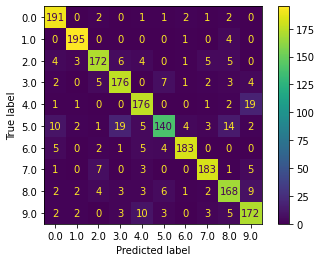
\includegraphics[width=\linewidth]{figure/logit_cm.png}
%   \caption{PCA}\label{fig:pca_none}
\endminipage\hfill
\minipage{0.24\textwidth}
  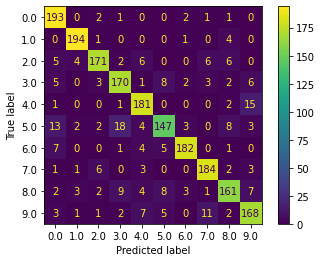
\includegraphics[width=\linewidth]{figure/logit_pca_cm.png}
%   \caption{kPCA}\label{fig:kpca_none}
\endminipage\hfill
\minipage{0.24\textwidth}
  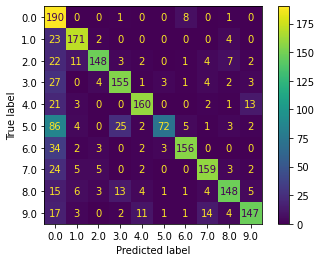
\includegraphics[width=\linewidth]{figure/logit_kpca_cm.png}
%   \caption{PCA}\label{fig:pca_none}
\endminipage\hfill
\minipage{0.24\textwidth}
  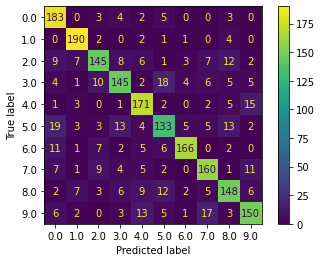
\includegraphics[width=\linewidth]{figure/logit_lda_cm.png}
%   \caption{kPCA}\label{fig:kpca_none}
\endminipage
\caption{Logistic Regression comfusion matrix for w/o dimensionality reduction, PCA, kPCA, LDA under (trial 1, feature extraction method 1)}
\label{logit_cm}
\end{figure}

From Figure~\ref{logit_cm}, we observe the following if we use the first feature extraction methods and do not apply the dimensionality reduction:
\begin{enumerate}
    \item w/o dimensionality reduction. 3 and 5, 4 and 9 are easily misclassified.
    \item PCA. 3 and 5, 4 and 9 are easily misclassified.
    \item kPCA. 0 and other digits are easily misclassified.
    \item LDA. 3 and 5, 0 and 5 are easily misclassified.
\end{enumerate}

Hence, generally, 3 and 5 should be a bottleneck for Logistic Regression no matter which combination of methods we are applying. Furthermore, we find that the reason for the underperformance of kPCA+Logistic Regression may be due to its loss of information to distinguish between 0 and other digits during the feature compression stage.

\subsubsection{Naive Bayes Classifier}
\emph{Remark: As there are in total 3 (number of methods of feature selections) $\times$ 4 (w/o, w/ 3 kinds of dimensionality reduction) $\times$ 2 (trials) = 24 possible combinations which are impossible to put all the figures within one report. For each parts where we insert figures, it use 4 figures, specifically, the figures under the condition w/o, w/ 3 kinds of dimensionality reduction when we use the first trial training data and the first feature extraction method to demonstrate the idea.}

\paragraph{Hyper-Parameter Tuning.}
We use \emph{Gaussian Naive Bayes Classifier} in this project. Regarding the prior, we adopt the default setting in \emph{Scikit-Learn} \cite{pedregosa2011scikit}, i.e., adjusted from the data, specifically in this case, $\frac{1}{C} = \frac{1}{10}$ for each class.

\paragraph{Results.}
Similarly, we use accuracy rate and confusion matrix as the metrics.

\begin{table}[!h]
\begin{tabular}{|c|c|ccc|}
\hline
\textit{\textbf{Algorithm}}                                                                    & \textit{\textbf{Num}}     & \multicolumn{3}{r|}{\textit{\textbf{Feature Extraction Method}}}                                                      \\ \hline
\textit{\textbf{GaussianNB}}                                                                   & \textit{\textbf{}}        & \multicolumn{1}{c|}{\textit{\textbf{1}}}     & \multicolumn{1}{c|}{\textit{\textbf{2}}}     & \textit{\textbf{3}}     \\ \hline
\multirow{3}{*}{\textit{\textbf{\begin{tabular}[c]{@{}c@{}}w/o dim\\ Reduction\end{tabular}}}} & \textit{\textbf{trial 1}} & \multicolumn{1}{c|}{\textit{\textbf{0.564}}} & \multicolumn{1}{c|}{\textit{\textbf{0.569}}} & \textit{\textbf{0.501}} \\ \cline{2-5} 
                                                                                               & \textit{\textbf{trial 2}} & \multicolumn{1}{c|}{\textit{\textbf{0.526}}} & \multicolumn{1}{c|}{\textit{\textbf{0.578}}} & \textit{\textbf{0.526}} \\ \cline{2-5} 
                                                                                               & \textit{\textbf{average}} & \multicolumn{1}{c|}{\textit{\textbf{0.545}}} & \multicolumn{1}{c|}{\textit{\textbf{0.574}}} & \textit{\textbf{0.514}} \\ \hline
\textit{\textbf{}}                                                                             & \textit{\textbf{trial 1}} & \multicolumn{1}{c|}{\textit{\textbf{0.784}}} & \multicolumn{1}{c|}{\textit{\textbf{0.774}}} & \textit{\textbf{0.770}} \\ \cline{2-5} 
\textit{\textbf{with PCA}}                                                                     & \textit{\textbf{trial 2}} & \multicolumn{1}{c|}{\textit{\textbf{0.776}}} & \multicolumn{1}{c|}{\textit{\textbf{0.780}}} & \textit{\textbf{0.766}} \\ \cline{2-5} 
\textit{\textbf{}}                                                                             & \textit{\textbf{average}} & \multicolumn{1}{c|}{\textit{\textbf{0.780}}} & \multicolumn{1}{c|}{\textit{\textbf{0.777}}} & \textit{\textbf{0.768}} \\ \hline
\textit{\textbf{}}                                                                             & \textit{\textbf{trial 1}} & \multicolumn{1}{c|}{\textit{\textbf{0.778}}} & \multicolumn{1}{c|}{\textit{\textbf{0.773}}} & \textit{\textbf{0.769}} \\ \cline{2-5} 
\textit{\textbf{with kPCA}}                                                                    & \textit{\textbf{trial 2}} & \multicolumn{1}{c|}{\textit{\textbf{0.764}}} & \multicolumn{1}{c|}{\textit{\textbf{0.763}}} & \textit{\textbf{0.767}} \\ \cline{2-5} 
\textit{\textbf{}}                                                                             & \textit{\textbf{average}} & \multicolumn{1}{c|}{\textit{\textbf{0.771}}} & \multicolumn{1}{c|}{\textit{\textbf{0.768}}} & \textit{\textbf{0.768}} \\ \hline
\textit{\textbf{}}                                                                             & \textit{\textbf{trial 1}} & \multicolumn{1}{c|}{\textit{\textbf{0.765}}} & \multicolumn{1}{c|}{\textit{\textbf{0.829}}} & \textit{\textbf{0.783}} \\ \cline{2-5} 
\textit{\textbf{with LDA}}                                                                     & \textit{\textbf{trial 2}} & \multicolumn{1}{c|}{\textit{\textbf{0.763}}} & \multicolumn{1}{c|}{\textit{\textbf{0.822}}} & \textit{\textbf{0.772}} \\ \cline{2-5} 
\textit{\textbf{}}                                                                             & \textit{\textbf{average}} & \multicolumn{1}{c|}{\textit{\textbf{0.764}}} & \multicolumn{1}{c|}{\textit{\textbf{\color{red}0.826}}} & \textit{\textbf{0.778}} \\ \hline
\end{tabular}
\caption{Results for Gaussian Naive Bayes Classifier}
\label{NB_res}
\end{table}

From Table~\ref{NB_res}, we conclude that for Gaussian Naive Bayes Classifier, if we use the second feature extraction methods, i.e. average over a $2 \times 2$ window of pixel values and apply LDA dimensionality reduction, we can get the best classification accuracy which is \textbf{0.826}.

\paragraph{Analysis for Gaussian Naive Bayes Classifier:}

\begin{enumerate}
    \item In general, Naive Bayes Classifier does not have a good performance, which may be due to we only have $n'=8000$ training data even after data augmentation which is not sufficient to train a generative model with too many parameters. On the hand, this also make the performance after dimensionality reduction much better (increased by around $0.2$ on average), since we significantly reduce the number of parameters.
    \item Regarding the feature extraction methods, we observe that all three methods tend to have similar performance if we do not apply dimensionality reduction, apply PCA or apply kPCA. Nevertheless, interestingly, it is noted that second feature extraction method (averaging over a $2 \times 2$ window of pixel values) significantly improve the performance if we apply LDA to the dataset.
\end{enumerate}

\paragraph{Confusion Matrix:}
Then we use confusion matrix to find out the most easily misclassified classes for Gaussian Naive Bayes Classifier.

\begin{figure}[!htb]
\minipage{0.24\textwidth}
  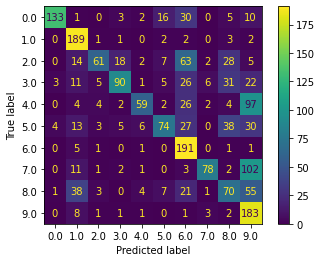
\includegraphics[width=\linewidth]{figure/nb.png}
%   \caption{PCA}\label{fig:pca_none}
\endminipage\hfill
\minipage{0.24\textwidth}
  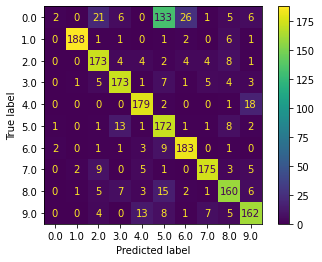
\includegraphics[width=\linewidth]{figure/nb_pca.png}
%   \caption{kPCA}\label{fig:kpca_none}
\endminipage\hfill
\minipage{0.24\textwidth}
  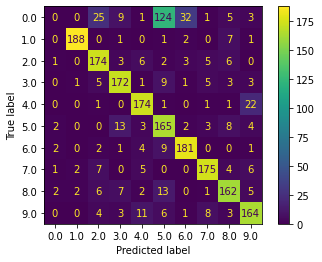
\includegraphics[width=\linewidth]{figure/nb_kpca.png}
%   \caption{PCA}\label{fig:pca_none}
\endminipage\hfill
\minipage{0.24\textwidth}
  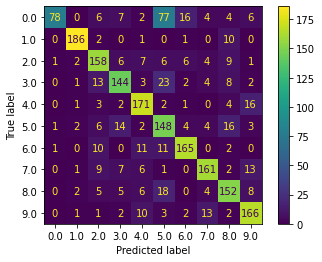
\includegraphics[width=\linewidth]{figure/nb_lda.png}
%   \caption{kPCA}\label{fig:kpca_none}
\endminipage
\caption{Gaussian Naive Bayes Classifier comfusion matrix for w/o dimensionality reduction, PCA, kPCA, LDA under (trial 1, feature extraction method 1)}
\label{nb_cm}
\end{figure}

From Figure~\ref{nb_cm}, we observe the following if we use the first feature extraction methods and do not apply the dimensionality reduction:
\begin{enumerate}
    \item w/o dimensionality reduction. 8 and 9, 4 and 9 are easily misclassified.
    \item PCA. 0 and 5 are easily misclassified.
    \item kPCA. 0 and 5 are easily misclassified.
    \item LDA. 0 and 5, 0 and 5 are easily misclassified.
\end{enumerate}

Hence, generally, 0 and 5 should be a bottleneck for Gaussian Naive Bayes Classifier if we apply any dimensionality reduction on it. However, from a human perspective, 0 and 5 should not be too difficult to distinguish between, we conjugate this may be due to the lack of data to train a stable model.

\subsubsection{Support Vector Machine}
\emph{Remark:}

\begin{enumerate}
    \item \emph{We will use rbf kernal for kSVM}
    \item As there are in total 3 (number of methods of feature selections) $\times$ 3 (w/ 3 kinds of dimensionality reduction) $\times$ 2 (trials) $\times$ 2 (linear SVM and SVM w/ kernel trick) = 36 possible combinations which are impossible to put all the figures within one report. For each parts where we insert figures, it use 6 figures, specifically, the figures under the condition w/ 3 kinds of dimensionality reduction combined with linear SVM and SVM w/ kernel trick when we use the first trial training data and the first feature extraction method to demonstrate the idea.
\end{enumerate}

\paragraph{Hyper-Parameter Tuning.}
Similar to Logistic Regression, we tune the inverse regularization parameter $C$.

\begin{figure}[!htb]
\minipage{0.24\textwidth}
  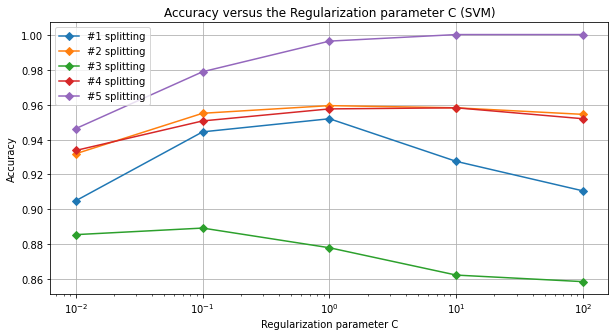
\includegraphics[width=\linewidth]{figure/svm.png}
%   \caption{PCA}\label{fig:pca_none}
\endminipage\hfill
\minipage{0.24\textwidth}
  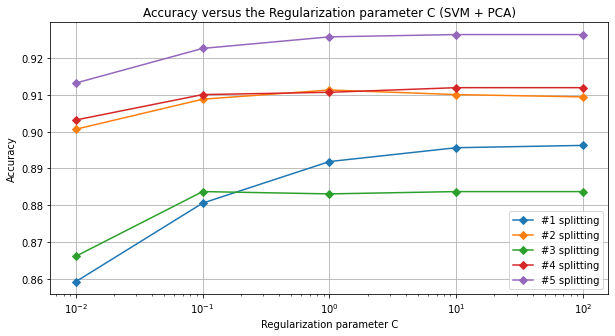
\includegraphics[width=\linewidth]{figure/svm_pca.png}
%   \caption{kPCA}\label{fig:kpca_none}
\endminipage\hfill
\minipage{0.24\textwidth}
  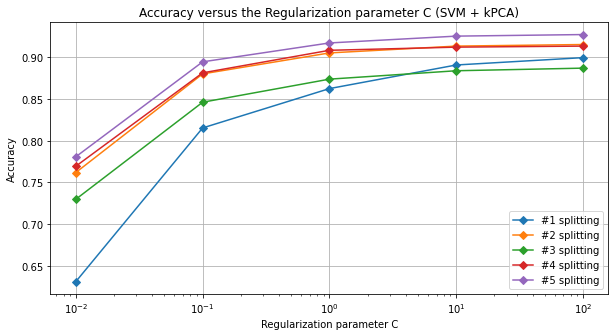
\includegraphics[width=\linewidth]{figure/svm_kpca.png}
%   \caption{PCA}\label{fig:pca_none}
\endminipage\hfill
\minipage{0.24\textwidth}
  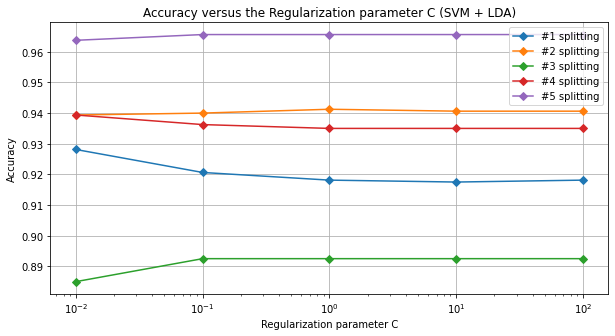
\includegraphics[width=\linewidth]{figure/svm_lda.png}
%   \caption{kPCA}\label{fig:kpca_none}
\endminipage
\caption{Linear Support Vector Machine hyper-parameter tuning for w/o dimensionality reduction, PCA, kPCA, LDA under (trial 1, feature extraction method 1)}
\label{lsvm_hyper}
\end{figure}

\begin{figure}[!htb]
\minipage{0.24\textwidth}
  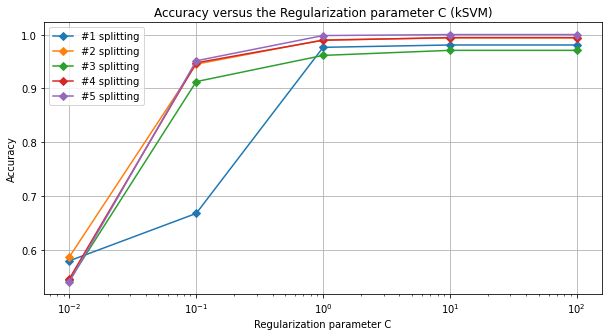
\includegraphics[width=\linewidth]{figure/ksvm.png}
%   \caption{PCA}\label{fig:pca_none}
\endminipage\hfill
\minipage{0.24\textwidth}
  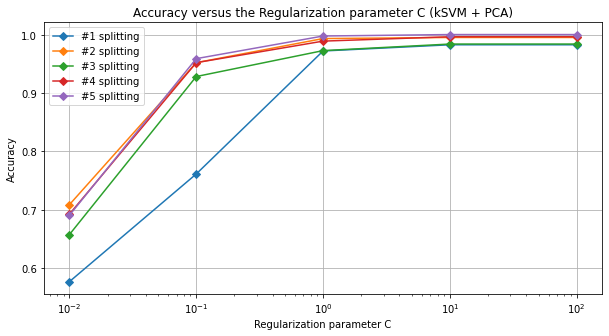
\includegraphics[width=\linewidth]{figure/ksvm_pca.png}
%   \caption{kPCA}\label{fig:kpca_none}
\endminipage\hfill
\minipage{0.24\textwidth}
  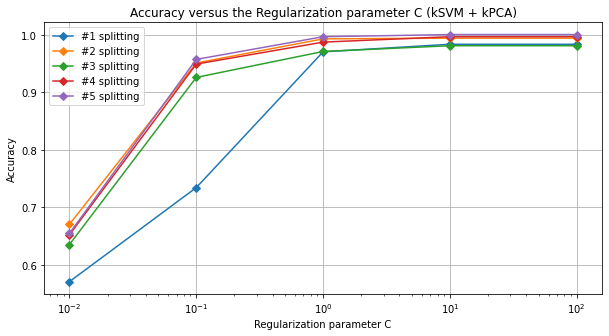
\includegraphics[width=\linewidth]{figure/ksvm_kpca.png}
%   \caption{PCA}\label{fig:pca_none}
\endminipage\hfill
\minipage{0.24\textwidth}
  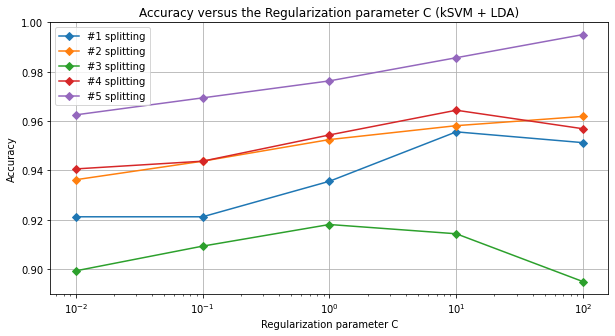
\includegraphics[width=\linewidth]{figure/ksvm_lda.png}
%   \caption{kPCA}\label{fig:kpca_none}
\endminipage
\caption{Support Vector Machine with rbf kernel hyper-parameter tuning for w/o dimensionality reduction, PCA, kPCA, LDA under (trial 1, feature extraction method 1)}
\label{ksvm_hyper}
\end{figure}

As we observe from Figure~\ref{lsvm_hyper} and Figure~\ref{ksvm_hyper}, the accuracy score on the cross-validation tends to increase as we increase the value of $C$. When the accuracy does not increase too much as $C$ increases, it indicates a higher chance of overfitting. Hence, for this particular case, we adopt $C = 1, 1, 1, 10$ for  w/o dimensionality reduction, PCA, kPCA, LDA, respectively for both SVM and kSVM. We adopt similar methods for other combination of trail and feature extraction methods.

\textbf{Results.}
% Please add the following required packages to your document preamble:
% \usepackage{multirow}
% \usepackage[table,xcdraw]{xcolor}
% If you use beamer only pass "xcolor=table" option, i.e. \documentclass[xcolor=table]{beamer}
\begin{table}[!htb]
\begin{tabular}{|c|c|ccc|}
\hline
\textit{\textbf{Algorithm}}                                                                     & \textit{\textbf{Num}}     & \multicolumn{3}{r|}{\textit{\textbf{Feature Extraction Method}}}                                                                                \\ \hline
\textit{\textbf{SVM}}                                                                           & \textit{\textbf{}}        & \multicolumn{1}{c|}{\textit{\textbf{1}}}                             & \multicolumn{1}{c|}{\textit{\textbf{2}}}      & \textit{\textbf{3}}      \\ \hline
                                                                                                & \textit{\textbf{trial 1}} & \multicolumn{1}{c|}{\textit{\textbf{0.8385}}}                        & \multicolumn{1}{c|}{\textit{\textbf{0.8795}}} & \textit{\textbf{0.805}}  \\ \cline{2-5} 
                                                                                                & \textit{\textbf{trial 2}} & \multicolumn{1}{c|}{\textit{\textbf{0.8375}}}                        & \multicolumn{1}{c|}{\textit{\textbf{0.8785}}} & \textit{\textbf{0.8035}} \\ \cline{2-5} 
\multirow{-3}{*}{\textit{\textbf{\begin{tabular}[c]{@{}c@{}}w/o dim\\ Reduction\end{tabular}}}} & \textit{\textbf{average}} & \multicolumn{1}{c|}{\textit{\textbf{0.838}}}                         & \multicolumn{1}{c|}{\textit{\textbf{0.879}}}  & \textit{\textbf{0.8043}} \\ \hline
\textit{\textbf{}}                                                                              & \textit{\textbf{trial 1}} & \multicolumn{1}{c|}{\textit{\textbf{0.8745}}}                        & \multicolumn{1}{c|}{\textit{\textbf{0.8825}}} & \textit{\textbf{0.8705}} \\ \cline{2-5} 
\textit{\textbf{with PCA}}                                                                      & \textit{\textbf{trial 2}} & \multicolumn{1}{c|}{\textit{\textbf{0.8625}}}                        & \multicolumn{1}{c|}{\textit{\textbf{0.8685}}} & \textit{\textbf{0.85}}   \\ \cline{2-5} 
\textit{\textbf{}}                                                                              & \textit{\textbf{average}} & \multicolumn{1}{c|}{\textit{\textbf{0.8685}}}                        & \multicolumn{1}{c|}{\textit{\textbf{0.8755}}} & \textit{\textbf{0.8288}} \\ \hline
\textit{\textbf{}}                                                                              & \textit{\textbf{trial 1}} & \multicolumn{1}{c|}{\textit{\textbf{0.8735}}}                        & \multicolumn{1}{c|}{\textit{\textbf{0.881}}}  & \textit{\textbf{0.871}}  \\ \cline{2-5} 
\textit{\textbf{with kPCA}}                                                                     & \textit{\textbf{trial 2}} & \multicolumn{1}{c|}{\textit{\textbf{0.8625}}}                        & \multicolumn{1}{c|}{\textit{\textbf{0.864}}}  & \textit{\textbf{0.855}}  \\ \cline{2-5} 
\textit{\textbf{}}                                                                              & \textit{\textbf{average}} & \multicolumn{1}{c|}{\textit{\textbf{0.868}}}                         & \multicolumn{1}{c|}{\textit{\textbf{0.8725}}} & \textit{\textbf{0.863}}  \\ \hline
\textit{\textbf{}}                                                                              & \textit{\textbf{trial 1}} & \multicolumn{1}{c|}{\textit{\textbf{0.8005}}}                        & \multicolumn{1}{c|}{\textit{\textbf{0.852}}}  & \textit{\textbf{0.8055}} \\ \cline{2-5} 
\textit{\textbf{with LDA}}                                                                      & \textit{\textbf{trial 2}} & \multicolumn{1}{c|}{\textit{\textbf{0.7785}}}                        & \multicolumn{1}{c|}{\textit{\textbf{0.8395}}} & \textit{\textbf{0.7995}} \\ \cline{2-5} 
\textit{\textbf{}}                                                                              & \textit{\textbf{average}} & \multicolumn{1}{c|}{\textit{\textbf{0.7895}}}                        & \multicolumn{1}{c|}{\textit{\textbf{0.846}}}  & \textit{\textbf{0.8025}} \\ \hline
\textit{\textbf{kSVM}}                                                                          & \textit{\textbf{}}        & \multicolumn{1}{c|}{\textit{\textbf{}}}                              & \multicolumn{1}{c|}{\textit{\textbf{}}}       & \textit{\textbf{}}       \\ \hline
                                                                                                & \textit{\textbf{trial 1}} & \multicolumn{1}{c|}{\textit{\textbf{0.9565}}}                        & \multicolumn{1}{c|}{\textit{\textbf{0.955}}}  & \textit{\textbf{0.9355}} \\ \cline{2-5} 
                                                                                                & \textit{\textbf{trial 2}} & \multicolumn{1}{c|}{\textit{\textbf{0.9505}}}                        & \multicolumn{1}{c|}{\textit{\textbf{0.9495}}} & \textit{\textbf{0.933}}  \\ \cline{2-5} 
\multirow{-3}{*}{\textit{\textbf{\begin{tabular}[c]{@{}c@{}}w/o dim\\ Reduction\end{tabular}}}} & \textit{\textbf{average}} & \multicolumn{1}{c|}{\textit{\textbf{0.9535}}}                        & \multicolumn{1}{c|}{\textit{\textbf{0.9523}}} & \textit{\textbf{0.9343}} \\ \hline
                                                                                                & \textit{\textbf{trial 1}} & \multicolumn{1}{c|}{\textit{\textbf{0.9585}}}                        & \multicolumn{1}{c|}{\textit{\textbf{0.959}}}  & \textit{\textbf{0.944}}  \\ \cline{2-5} 
                                                                                                & \textit{\textbf{trial 2}} & \multicolumn{1}{c|}{\textit{\textbf{0.956}}}                         & \multicolumn{1}{c|}{\textit{\textbf{0.951}}}  & \textit{\textbf{0.9445}} \\ \cline{2-5} 
\multirow{-3}{*}{\textit{\textbf{with PCA}}}                                                    & \textit{\textbf{average}} & \multicolumn{1}{c|}{{\color[HTML]{FE0000} \textit{\textbf{0.9573}}}} & \multicolumn{1}{c|}{\textit{\textbf{0.955}}}  & \textit{\textbf{0.9443}} \\ \hline
                                                                                                & \textit{\textbf{trial 1}} & \multicolumn{1}{c|}{\textit{\textbf{0.9575}}}                        & \multicolumn{1}{c|}{\textit{\textbf{0.9575}}} & \textit{\textbf{0.9435}} \\ \cline{2-5} 
                                                                                                & \textit{\textbf{trial 2}} & \multicolumn{1}{c|}{\textit{\textbf{0.9525}}}                        & \multicolumn{1}{c|}{\textit{\textbf{0.9485}}} & \textit{\textbf{0.9415}} \\ \cline{2-5} 
\multirow{-3}{*}{\textit{\textbf{with kPCA}}}                                                   & \textit{\textbf{average}} & \multicolumn{1}{c|}{\textit{\textbf{0.955}}}                         & \multicolumn{1}{c|}{\textit{\textbf{0.953}}}  & \textit{\textbf{0.9425}} \\ \hline
                                                                                                & \textit{\textbf{trial 1}} & \multicolumn{1}{c|}{\textit{\textbf{0.819}}}                         & \multicolumn{1}{c|}{\textit{\textbf{0.8775}}} & \textit{\textbf{0.819}}  \\ \cline{2-5} 
                                                                                                & \textit{\textbf{trial 2}} & \multicolumn{1}{c|}{\textit{\textbf{0.7895}}}                        & \multicolumn{1}{c|}{\textit{\textbf{0.862}}}  & \textit{\textbf{0.817}}  \\ \cline{2-5} 
\multirow{-3}{*}{\textit{\textbf{with LDA}}}                                                    & \textit{\textbf{average}} & \multicolumn{1}{c|}{\textit{\textbf{0.804}}}                         & \multicolumn{1}{c|}{\textit{\textbf{0.8698}}} & \textit{\textbf{0.818}}  \\ \hline
\end{tabular}
\caption{Results for Support Vector Machine}
\label{SVM_res}
\end{table}

From Table~\ref{SVM_res}, we conclude that for Support Vector Machine, If we use the first feature extraction method, i.e. directly use the original features, and apply PCA, we can get the best classification accuracy which is \textbf{0.9573}.

\paragraph{Analysis for Support Vector Machine:}

\begin{enumerate}
    \item In general, compared with other traditional machine learning algorithms, SVM tends to perform better.
    \item Regarding the feature extraction methods, we observe that method 1 tends to give the best performance which is different from logistic regression and naive bayes classifier. We conjugate this may due to SVM can use few data to train a model with many features.
    \item Compared with w/o dimensionality reduction and LDA, PCA and kPCA can give better performance in this case.
\end{enumerate}

\paragraph{Confusion Matrix:}
Then we use confusion matrix to find out the most easily misclassified classes for Support Vector Machine.

\begin{figure}[!htb]
\minipage{0.24\textwidth}
  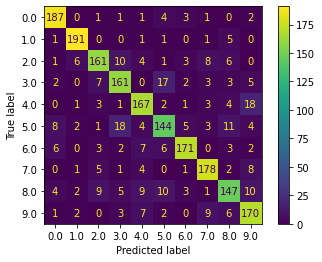
\includegraphics[width=\linewidth]{figure/svm_cm.png}
%   \caption{PCA}\label{fig:pca_none}
\endminipage\hfill
\minipage{0.24\textwidth}
  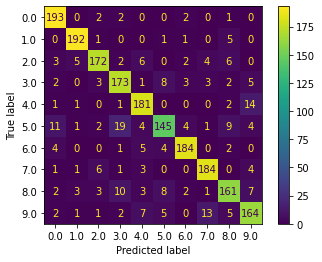
\includegraphics[width=\linewidth]{figure/svm_pca_cm.png}
%   \caption{kPCA}\label{fig:kpca_none}
\endminipage\hfill
\minipage{0.24\textwidth}
  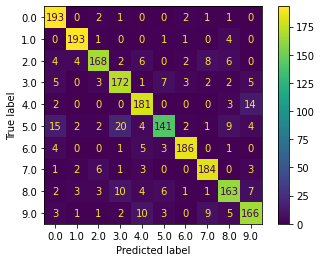
\includegraphics[width=\linewidth]{figure/svm_kpca_cm.png}
%   \caption{PCA}\label{fig:pca_none}
\endminipage\hfill
\minipage{0.24\textwidth}
  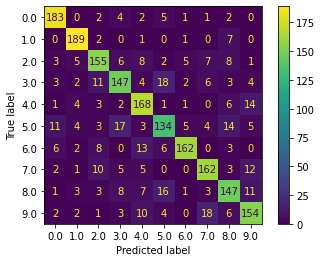
\includegraphics[width=\linewidth]{figure/svm_lda_cm.png}
%   \caption{kPCA}\label{fig:kpca_none}
\endminipage
\caption{Linear SVM comfusion matrix for w/o dimensionality reduction, PCA, kPCA, LDA under (trial 1, feature extraction method 1)}
\label{lsvm_cm}
\end{figure}

\begin{figure}[!htb]
\minipage{0.24\textwidth}
  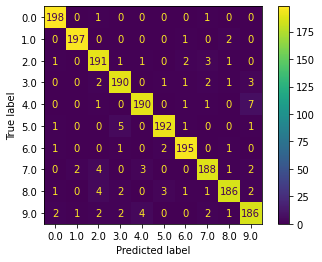
\includegraphics[width=\linewidth]{figure/ksvm_cm.png}
%   \caption{PCA}\label{fig:pca_none}
\endminipage\hfill
\minipage{0.24\textwidth}
  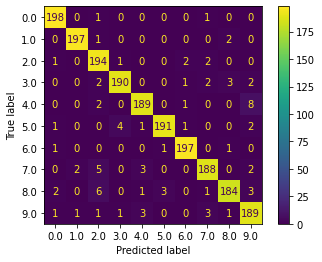
\includegraphics[width=\linewidth]{figure/ksvm_pca_cm.png}
%   \caption{kPCA}\label{fig:kpca_none}
\endminipage\hfill
\minipage{0.24\textwidth}
  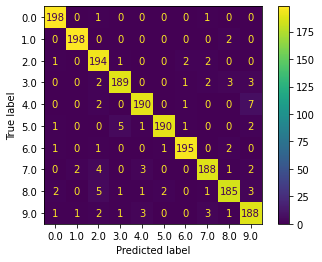
\includegraphics[width=\linewidth]{figure/ksvm_kpca_cm.png}
%   \caption{PCA}\label{fig:pca_none}
\endminipage\hfill
\minipage{0.24\textwidth}
  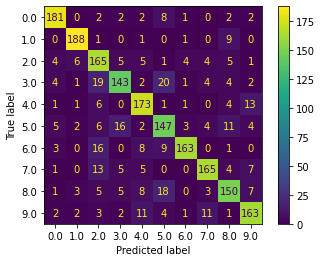
\includegraphics[width=\linewidth]{figure/ksvm_lda_cm.png}
%   \caption{kPCA}\label{fig:kpca_none}
\endminipage
\caption{SVM with rbf kernel comfusion matrix for w/o dimensionality reduction, PCA, kPCA, LDA under (trial 1, feature extraction method 1)}
\label{ksvm_cm}
\end{figure}

From Figure~\ref{lsvm_cm}, we observe the following if we use the first feature extraction methods and do not apply the dimensionality reduction:
\begin{enumerate}
    \item SVM+w/o dimensionality reduction. 3 and 5, 4 and 9 are easily misclassified.
    \item SVM+PCA. 3 and 5, 4 and 9 are easily misclassified.
    \item SVM+kPCA. 3 and 5, 4 and 9 are easily misclassified.
    \item SVM+LDA. 3 and 5, 4 and 9 are easily misclassified.
\end{enumerate}

Moreover, From Figure~\ref{ksvm_cm}, we observe the following:
\begin{enumerate}
    \item SVM+w/o dimensionality reduction. 3 and 5 are easily misclassified.
    \item SVM+PCA. 3 and 5 are easily misclassified.
    \item SVM+kPCA.3 and 5 are easily misclassified.
    \item SVM+LDA. 3 and 5, 5 and 8 are easily misclassified.
\end{enumerate}

Hence, generally, 3 and 5 should be a bottleneck for Support Vector Machine. 
\subsubsection{Muilti-Layer Perceptron}
\emph{Remark: For neural network part, we didn't show hyper-parameter tuning results for the MLP network as it's prone to overfitting and omits local information in the image as mentioned in Section~\ref{nn}. Due to these limitations, the effect of hyper-parameter tuning is not significant.} 
\paragraph{Experiment Setup. } As presented in Figure~\ref{nn_demo} in Appendix~\ref{}, we constructed a simple neural network containing four fully-connected layers.  

Following \cite{ensemble}, we added a batch normalization layer after each dense layer to prevent overfitting. For the hyper-parameters we set a relatively low learning rate of 0.01 with a decay rate = 1e-6 and used a Stochastic Gradient Descent Optimizer with momentum = 0.9 to train the model for 40 epochs. 
\paragraph{Results. } 
\begin{table}[!htb]
\centering
\begin{tabular}{|c|c|c|}
\hline

\textit{\textbf{Algorithm}}                                                                    & \textit{\textbf{Num}}     & \multicolumn{1}{c|}{\textit{\textbf{Test Accuracy}}}                                                        \\ \hline

\multirow{3}{*}{\textit{\textbf{\begin{tabular}[c]{@{}c@{}}MLP
\end{tabular}}}} & \textit{\textbf{trial 1}} & \multicolumn{1}{c|}{\textit{\textbf{0.94}}}
  \\ \cline{2-3} 
                                                                                               & \textit{\textbf{trial 2}} &  \multicolumn{1}{c|}{\textit{\textbf{0.9375}}}  \\ \cline{2-3} 
                                                                                               & \textit{\textbf{average}} &  \multicolumn{1}{c|}{\textit{\textbf{0.9388}}} \\ \hline
\end{tabular}
\caption{Results for Multi-Layer Perceptron}
\label{MLP_res}
\end{table}
For each portion of the data, we run an experiments to get the performance on the test data as shown in Table~\ref{MLP_res}. As shwon in Figure~\ref{mlp_train}, we can find that the model converge fairly fast during the training and the accuracy is close to 1.0 at the end. The test accuracy is only 0.938 on average, which is a indication of overfitting. 

\begin{figure}[h]
\centering{}
  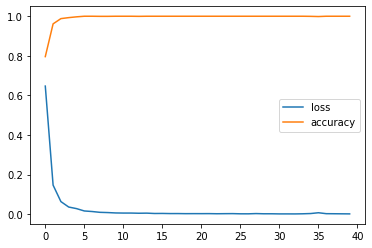
\includegraphics[width=0.4\textwidth]{figure/MLP_Train.png}
  \caption{Training Process}
  \label{mlp_train}
\end{figure}

\subsubsection{Convolutional Neural Network}
\paragraph{Experiment Setup. }
Following \cite{ensemble}, our network models consist of multiple convolution layers and a fully connected layer to output the class labels at the end. In each convolution layer, a 2D convolution is performed, followed by batch normalization and ReLU activation. Pooling layer is not used after convolution. Instead, the size of feature map is reduced after each convolution because padding is not used. For example, if we use a 3×3 kernel, the width and height of the image is reduced by two after each convolution layer. This setting is proved to have better performance than the traditional CNN network with pooling layer. Following this design, we construct four networks in total. The first three networks has different filter size: 3x3, 5x5, and 7x7, which also resulting in different number of layers since the rate of dimension reduction in feature map varies. The first network in Figure~\ref{cnn_m3_demo} in Appendix~\ref{cnn_3}, M3, uses 11 convolution layers with 16i channels in ith convolution layer. The feature map becomes 14x14 with 176 channels after the 11th layer. The second network M5 in Figure~\ref{cnn_m5_demo} in Appendix~\ref{cnn_5} has 6 convolution layers. The feature map becomes 14×14 with 176 channels after the 6th layer. The third network M7 in Figure~\ref{cnn_m7_demo} in Appendix~\ref{cnn_7} has 4 convolution layers with 48i channels in ith convolution layer. The feature map becomes 12×12 with 192 channels after the 4th layer. The last network is an ensemble of the three models using majority voting. There are two ways of voting: hard voting and soft voting. For hard voting, we simply take the modes of the output from the three single network and randomly choose one if the three models all has different result. For soft voting, we average the probability returned by the softmax function in the last layer and treat it as the output from a single model. In cite{ensemble}, they used a hard voting to assign the label yet we are also curious about the performance of soft voting.

Before entering the convolutional layer, we added a resize layer to resize the image from 28x28 to 36x36 as we found the image with original size may have limited information for training. For validation, we split the original training set into training data and validation data in the proportion of 9 : 1. We set the learning rate to be 0.001 and used Adam with a decay of 1e-6 for M3 and M5 training and RMSprop with momentum = 0.9, epsilon = 0.1 for M7 training. To prevent overfitting, we also used a early stopping with patience = 20 to stop the training once the model converges. The training epoch is set to 120.


\paragraph{Results. }
Since the network is stochastic, we run five independent experiments with different seeds and take the averaged result as an indication of performance. The best performance on test set and challenge set are both given by Soft Voting. From the Figure~\ref{cnn_box}, we can also see that the soft voting can maintain a relatively low variance over other models. For the three models without ensemble, we can see that filter size 7x7 has a better performance which is also explainable as a small size window cannot catch the feature of the digit easily.  For the two ensemble models, we can see that soft voting is better and has lower variance which is also explainable as soft voting is more robust to the abnormal output.

% Please add the following required packages to your document preamble:
% \usepackage{multirow}
% \usepackage[table,xcdraw]{xcolor}
% If you use beamer only pass "xcolor=table" option, i.e. \documentclass[xcolor=table]{beamer}
\begin{table}[]
\begin{tabular}{|c|c|cc|}
\hline
\textit{\textbf{Algorithm}}                     & \textit{\textbf{Num}}     & \multicolumn{2}{c|}{\textit{\textbf{Accuracy}}}                                                                      \\ \hline
\multicolumn{1}{|l|}{}                          & \multicolumn{1}{l|}{}     & \multicolumn{1}{c|}{Test}                                           & Challenge                                      \\ \hline
\textit{\textbf{M3}}                            & \textit{\textbf{Trial 1}} & \multicolumn{1}{c|}{\textit{\textbf{98.20 (0.41)}}}                 & \textit{\textbf{92.80 (1.60)}}                 \\ \cline{2-4} 
\textit{\textbf{}}                              & \textit{\textbf{Trial 2}} & \multicolumn{1}{c|}{\textit{\textbf{98.06(0.27)}}}                  & \textit{\textbf{93.33 (0.73)}}                 \\ \cline{2-4} 
\textit{\textbf{}}                              & \textit{\textbf{Average}} & \multicolumn{1}{c|}{\textit{\textbf{98.13}}}                        & \textit{\textbf{93.05}}                        \\ \hline
                                                & \textit{\textbf{Trial 1}} & \multicolumn{1}{c|}{\textit{\textbf{98.51 (0.12)}}}                 & \textit{\textbf{94.1 (0.98)}}                  \\ \cline{2-4} 
                                                & \textit{\textbf{Trial 2}} & \multicolumn{1}{c|}{\textit{\textbf{98.21 (0.30)}}}                 & \textit{\textbf{92.40 (3.39)}}                 \\ \cline{2-4} 
\multirow{-3}{*}{\textit{\textbf{M5}}}          & \textit{\textbf{Average}} & \multicolumn{1}{c|}{\textit{\textbf{98.31}}}                        & \textit{\textbf{93.25}}                        \\ \hline
                                                & \textit{\textbf{Trial 1}} & \multicolumn{1}{c|}{\textit{\textbf{98.41 (0.27)}}}                 & \textit{\textbf{94.8 (0.88)}}                  \\ \cline{2-4} 
                                                & \textit{\textbf{Trial 2}} & \multicolumn{1}{c|}{\textit{\textbf{98.32 (0.19)}}}                 & \textit{\textbf{94.67(1.12)}}                  \\ \cline{2-4} 
\multirow{-3}{*}{\textit{\textbf{M7}}}          & \textit{\textbf{Average}} & \multicolumn{1}{c|}{\textit{\textbf{98.37}}}                        & {\color[HTML]{333333} \textit{\textbf{94.74}}} \\ \hline
                                                & \textit{\textbf{Trial 1}} & \multicolumn{1}{c|}{\textit{\textbf{98.99 (0.30)}}}                 & \textit{\textbf{94.8 (0.27)}}                  \\ \cline{2-4} 
                                                & \textit{\textbf{Trial 2}} & \multicolumn{1}{c|}{\textit{\textbf{98.56 (0.09)}}}                 & \textit{\textbf{94.67 (1.33)}}                 \\ \cline{2-4} 
\multirow{-3}{*}{\textit{\textbf{Soft Voting}}} & \textit{\textbf{Average}} & \multicolumn{1}{c|}{{\color[HTML]{FE0000} \textit{\textbf{98.78}}}} & {\color[HTML]{FE0000} \textit{\textbf{94.74}}} \\ \hline
                                                & \textit{\textbf{Trial 1}} & \multicolumn{1}{c|}{\textit{\textbf{98.65 (0.19)}}}                 & \textit{\textbf{93.6 (1.77)}}                  \\ \cline{2-4} 
                                                & \textit{\textbf{Trial 2}} & \multicolumn{1}{c|}{\textit{\textbf{98.34 (0.18)}}}                 & \textit{\textbf{94.53 (0.27)}}                 \\ \cline{2-4} 
\multirow{-3}{*}{\textit{\textbf{Hard Voting}}} & \textit{\textbf{Average}} & \multicolumn{1}{c|}{\textit{\textbf{98.50}}}                        & \textit{\textbf{94.07}}                        \\ \hline
\end{tabular}
\end{table}


\begin{figure}[!htb]
\minipage{0.24\textwidth}
  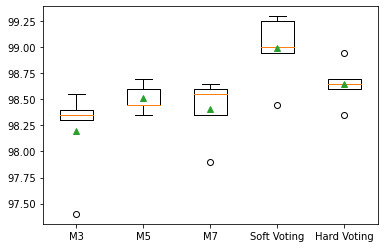
\includegraphics[width=\linewidth]{figure/cnn_test_1.png}

\endminipage\hfill
\minipage{0.24\textwidth}
  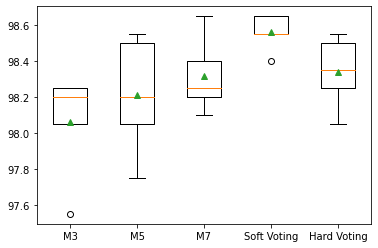
\includegraphics[width=\linewidth]{figure/cnn_test_2.png}
\endminipage\hfill
\minipage{0.24\textwidth}
  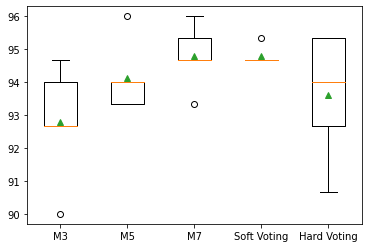
\includegraphics[width=\linewidth]{figure/cnn_challenge_1.png}
\endminipage\hfill
\minipage{0.24\textwidth}
  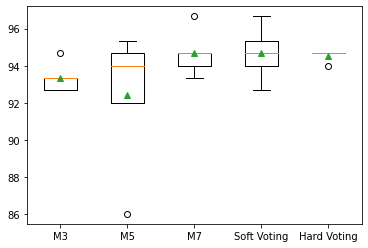
\includegraphics[width=\linewidth]{figure/cnn_challenge_2.png}
\endminipage\hfill
\caption{Accuracy boxplot on test and challenge tests. The first row is the test result on two different portion of training data respectively and the second row is the challenge test result also on two different training data)}
\label{cnn_box}
\end{figure}

\paragraph{Effect of Data Augmentation. } \label{aug_survey}
In this section, we try to investigate the effect of data augmentation as mentioned in Section~\ref{aug}. Since the performance of the five models don't have a large distinction, we use model M7 as a illustration as it has the best performance on single model and can save the cost of training compared with ensemble model. From Table~\ref{aug_res} and Figure~\ref{aug_box}, we can see that internal augmentation has a better performance. This is a counter-example for "more data is better" as external augmentation add 6000 more examples while worsening the results. 


% Please add the following required packages to your document preamble:
% \usepackage{multirow}
% \usepackage[table,xcdraw]{xcolor}
% If you use beamer only pass "xcolor=table" option, i.e. \documentclass[xcolor=table]{beamer}
\begin{table}[!htb]
\begin{tabular}{|c|c|cc|}
\hline
\textit{\textbf{Algorithm}}                                                                         & \textit{\textbf{Num}}     & \multicolumn{2}{c|}{\textit{\textbf{Accuracy}}}                                                                      \\ \hline
\multicolumn{1}{|l|}{}                                                                              & \multicolumn{1}{l|}{}     & \multicolumn{1}{c|}{Test}                                           & Challenge                                      \\ \hline
                                                                                                    & \textit{\textbf{Trial 1}} & \multicolumn{1}{c|}{\textit{\textbf{98.25 (0.39)}}}                 & \textit{\textbf{96.40 (0.90)}}                  \\ \cline{2-4} 
                                                                                                    & \textit{\textbf{Trial 2}} & \multicolumn{1}{c|}{\textit{\textbf{98.12 (0.27)}}}                 & \textit{\textbf{93.73 (1.44)}}                 \\ \cline{2-4} 
\multirow{-3}{*}{\textit{\textbf{\begin{tabular}[c]{@{}c@{}}Internal\\ Augmentation\end{tabular}}}} & \textit{\textbf{Average}} & \multicolumn{1}{c|}{{\color[HTML]{FE0000} \textit{\textbf{98.19}}}} & {\color[HTML]{FE0000} \textit{\textbf{95.07}}} \\ \hline
                                                                                                    & \textit{\textbf{Trial 1}} & \multicolumn{1}{c|}{\textit{\textbf{97.12 (0.19)}}}                 & \textit{\textbf{81.20(1.42)}}                  \\ \cline{2-4} 
                                                                                                    & \textit{\textbf{Trial 2}} & \multicolumn{1}{c|}{\textit{\textbf{97.36 (0.21)}}}                 & \textit{\textbf{85.20 (0.78)}}                 \\ \cline{2-4} 
\multirow{-3}{*}{\textit{\textbf{\begin{tabular}[c]{@{}c@{}}External\\ Augmentation\end{tabular}}}} & \textit{\textbf{Average}} & \multicolumn{1}{c|}{\textit{\textbf{97.24}}}                        & \textit{\textbf{83.2}}                        \\ \hline
\end{tabular}
\label{aug_res}
\end{table}







\begin{figure}[!htb]
\minipage{0.24\textwidth}
  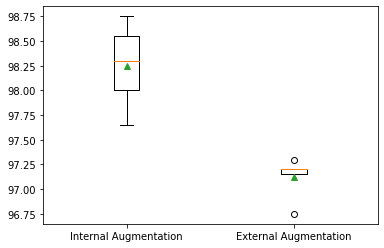
\includegraphics[width=\linewidth]{figure/aug_test_1.png}

\endminipage\hfill
\minipage{0.24\textwidth}
  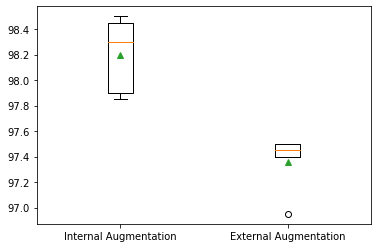
\includegraphics[width=\linewidth]{figure/aug_test_2.png}
\endminipage\hfill
\minipage{0.24\textwidth}
  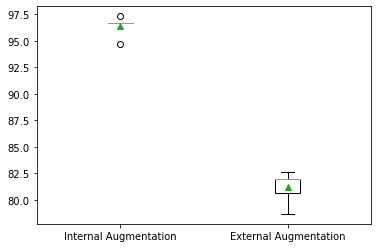
\includegraphics[width=\linewidth]{figure/aug_challenge_1.png}
\endminipage\hfill
\minipage{0.24\textwidth}
  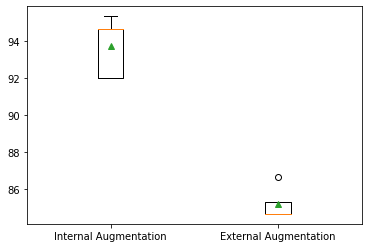
\includegraphics[width=\linewidth]{figure/aug_challenge_2.png}
\endminipage\hfill
\caption{Accuracy boxplot on test and challenge tests. The first row is the test result on two different portion of training data respectively and the second row is the challenge test result also on two different training data)}
\label{aug_box}
\end{figure}

\section{Conclusion}
\subsection{Traditional Machine Learning Algorithms}
We conclude that there is no single silver bullet for feature selection method, dimensionality reduction method or classification method even on this single MNIST dataset. For example, feature selection method 2 may perform well when we use Logistic Regression and Naive Bayes Classifier, but feature selection method 1 performs much better when SVM is applied. Hence, it is crucial in to select the pre-processing technics used for each classification methods. 

We also note here that within all traditional machine learning algorithms we use in this project, the best performance we achieve is \textbf{0.9573}. 
\subsection{Neural Networks}
We can draw our findings mainly in three perspectives. First, CNN has a better performance over simple MLP as it can extract more features using filter window. Second, we implemented an ensemble model to boost our performance from single model as model with different window size can focus on different features, which as a result they made errors on slightly different sample. Notably, an ensemble network can only be implemented when the performances between single networks don't vary largely otherwise the "bad student" will drag the "good student" to poor performance. Lastly, we inspected on the effect on the augmentation techniques. Data augmentation is usually used for preventing overfitting. CNN is also prone to overfit thus we intend to use it as a tool to boost the performance. Surprisingly we find adding more samples will make the model has a worse performance. Though the augmentation setting have some slightly difference between the two ways, yet we can still draw the conclusion that augmenting on the original data may help the model grasp the features better. For future work, we may need to verify this conclusion on more models to make it more solid. For the limitation of the work, by inspecting the failed samples, we found the network cannot distinguish '9' and '7' easily. This problem may be solved with more samples

% \LaTeX{} and Word style files that implement these instructions
% can be retrieved electronically. (See Appendix~\ref{stylefiles} for
% instructions on how to obtain these files.)

% \subsection{Layout}

% Print manuscripts two columns to a page, in the manner in which these
% instructions are printed. The exact dimensions for pages are:
% \begin{itemize}
% \item left and right margins: .75$''$
% \item column width: 3.375$''$
% \item gap between columns: .25$''$
% \item top margin---first page: 1.375$''$
% \item top margin---other pages: .75$''$
% \item bottom margin: 1.25$''$
% \item column height---first page: 6.625$''$
% \item column height---other pages: 9$''$
% \end{itemize}

% All measurements assume an 8-1/2$''$ $\times$ 11$''$ page size. For
% A4-size paper, use the given top and left margins, column width,
% height, and gap, and modify the bottom and right margins as necessary.

% \subsection{Format of Electronic Manuscript}

% For the production of the electronic manuscript, you must use Adobe's
% {\em Portable Document Format} (PDF). A PDF file can be generated, for
% instance, on Unix systems using {\tt ps2pdf} or on Windows systems
% using Adobe's Distiller. There is also a website with free software
% and conversion services: \url{http://www.ps2pdf.com}. For reasons of
% uniformity, use of Adobe's {\em Times Roman} font is strongly suggested.
% In \LaTeX2e{} this is accomplished by writing
% \begin{quote}
% \mbox{\tt $\backslash$usepackage\{times\}}
% \end{quote}
% in the preamble.\footnote{You may want also to use the package {\tt
% latexsym}, which defines all symbols known from the old \LaTeX{}
% version.}

% Additionally, it is of utmost importance to specify the {\bf
% letter} format (corresponding to 8-1/2$''$ $\times$ 11$''$) when
% formatting the paper. When working with {\tt dvips}, for instance, one
% should specify {\tt -t letter}.

% \subsection{Title and Author Information}

% Center the title on the entire width of the page in a 14-point bold
% font. The title must be capitalized using Title Case. Below it, center author name(s) in 12-point bold font. On the following line(s) place the affiliations, each affiliation on its own line using 12-point regular font. Matching between authors and affiliations can be done using numeric superindices. Optionally, a comma-separated list of email addresses follows the affiliation(s) line(s), using 12-point regular font.

% \subsubsection{Blind Review}

% In order to make blind reviewing possible, authors must omit their
% names and affiliations when submitting the paper for review. In place
% of names and affiliations, provide a list of content areas. When
% referring to one's own work, use the third person rather than the
% first person. For example, say, ``Previously,
% Gottlob~\shortcite{gottlob:nonmon} has shown that\ldots'', rather
% than, ``In our previous work~\cite{gottlob:nonmon}, we have shown
% that\ldots'' Try to avoid including any information in the body of the
% paper or references that would identify the authors or their
% institutions. Such information can be added to the final camera-ready
% version for publication.

% \subsection{Abstract}

% Place the abstract at the beginning of the first column 3$''$ from the
% top of the page, unless that does not leave enough room for the title
% and author information. Use a slightly smaller width than in the body
% of the paper. Head the abstract with ``Abstract'' centered above the
% body of the abstract in a 12-point bold font. The body of the abstract
% should be in the same font as the body of the paper.

% The abstract should be a concise, one-paragraph summary describing the
% general thesis and conclusion of your paper. A reader should be able
% to learn the purpose of the paper and the reason for its importance
% from the abstract. The abstract should be no more than 200 words long.

% \subsection{Text}

% The main body of the text immediately follows the abstract. Use
% 10-point type in a clear, readable font with 1-point leading (10 on
% 11).

% Indent when starting a new paragraph, except after major headings.

% \subsection{Headings and Sections}

% When necessary, headings should be used to separate major sections of
% your paper. (These instructions use many headings to demonstrate their
% appearance; your paper should have fewer headings.). All headings should be capitalized using Title Case.

% \subsubsection{Section Headings}

% Print section headings in 12-point bold type in the style shown in
% these instructions. Leave a blank space of approximately 10 points
% above and 4 points below section headings.  Number sections with
% arabic numerals.

% \subsubsection{Subsection Headings}

% Print subsection headings in 11-point bold type. Leave a blank space
% of approximately 8 points above and 3 points below subsection
% headings. Number subsections with the section number and the
% subsection number (in arabic numerals) separated by a
% period.

% \subsubsection{Subsubsection Headings}

% Print subsubsection headings in 10-point bold type. Leave a blank
% space of approximately 6 points above subsubsection headings. Do not
% number subsubsections.

% \paragraph{Titled paragraphs.} You should use titled paragraphs if and
% only if the title covers exactly one paragraph. Such paragraphs should be
% separated from the preceding content by at least 3pt, and no more than
% 6pt. The title should be in 10pt bold font and ended with a period.
% After that, a 1em horizontal space should follow the title before
% the paragraph's text.

% In \LaTeX{} titled paragraphs should be typeset using
% \begin{quote}
% {\tt \textbackslash{}paragraph\{Title.\} text} .
% \end{quote}

% \subsubsection{Acknowledgements}

% You may include an unnumbered acknowledgments section, including
% acknowledgments of help from colleagues, financial support, and
% permission to publish. If present, acknowledgements must be in a dedicated,
% unnumbered section appearing after all regular sections but before any
% appendices or references.

% Use
% \begin{quote}
%     {\tt \textbackslash{}section*\{Acknowledgements\}})
% \end{quote}
% to typeset the acknowledgements section in \LaTeX{}.

% \subsubsection{Appendices}

% Any appendices directly follow the text and look like sections, except
% that they are numbered with capital letters instead of arabic
% numerals. See this document for an example.

% \subsubsection{References}

% The references section is headed ``References'', printed in the same
% style as a section heading but without a number. A sample list of
% references is given at the end of these instructions. Use a consistent
% format for references. The reference list should not include publicly unavailable work.

% \subsection{Citations}

% Citations within the text should include the author's last name and
% the year of publication, for example~\cite{gottlob:nonmon}.  Append
% lowercase letters to the year in cases of ambiguity.  Treat multiple
% authors as in the following examples:~\cite{abelson-et-al:scheme}
% or~\cite{bgf:Lixto} (for more than two authors) and
% \cite{brachman-schmolze:kl-one} (for two authors).  If the author
% portion of a citation is obvious, omit it, e.g.,
% Nebel~\shortcite{nebel:jair-2000}.  Collapse multiple citations as
% follows:~\cite{gls:hypertrees,levesque:functional-foundations}.
% \nocite{abelson-et-al:scheme}
% \nocite{bgf:Lixto}
% \nocite{brachman-schmolze:kl-one}
% \nocite{gottlob:nonmon}
% \nocite{gls:hypertrees}
% \nocite{levesque:functional-foundations}
% \nocite{levesque:belief}
% \nocite{nebel:jair-2000}

% \subsection{Footnotes}

% Place footnotes at the bottom of the page in a 9-point font.  Refer to
% them with superscript numbers.\footnote{This is how your footnotes
% should appear.} Separate them from the text by a short
% line.\footnote{Note the line separating these footnotes from the
% text.} Avoid footnotes as much as possible; they interrupt the flow of
% the text.

% \section{Illustrations}

% Place all illustrations (figures, drawings, tables, and photographs)
% throughout the paper at the places where they are first discussed,
% rather than at the end of the paper.

% They should be floated to the top (preferred) or bottom of the page,
% unless they are an integral part
% of your narrative flow. When placed at the bottom or top of
% a page, illustrations may run across both columns, but not when they
% appear inline.

% Illustrations must be rendered electronically or scanned and placed
% directly in your document. They should be cropped outside \LaTeX{},
% otherwise portions of the image could reappear during the post-processing of your paper.
% When possible, generate your illustrations in a vector format.
% When using bitmaps, please use 300dpi resolution at least.
% All illustrations should be understandable when printed in black and
% white, albeit you can use colors to enhance them. Line weights should
% be 1/2-point or thicker. Avoid screens and superimposing type on
% patterns, as these effects may not reproduce well.

% Number illustrations sequentially. Use references of the following
% form: Figure 1, Table 2, etc. Place illustration numbers and captions
% under illustrations. Leave a margin of 1/4-inch around the area
% covered by the illustration and caption.  Use 9-point type for
% captions, labels, and other text in illustrations. Captions should always appear below the illustration.

% \section{Tables}

% Tables are considered illustrations containing data. Therefore, they should also appear floated to the top (preferably) or bottom of the page, and with the captions below them.

% \begin{table}
% \centering
% \begin{tabular}{lll}
% \hline
% Scenario  & $\delta$ & Runtime \\
% \hline
% Paris       & 0.1s  & 13.65ms     \\
% Paris       & 0.2s  & 0.01ms      \\
% New York    & 0.1s  & 92.50ms     \\
% Singapore   & 0.1s  & 33.33ms     \\
% Singapore   & 0.2s  & 23.01ms     \\
% \hline
% \end{tabular}
% \caption{Latex default table}
% \label{tab:plain}
% \end{table}

% \begin{table}
% \centering
% \begin{tabular}{lrr}
% \toprule
% Scenario  & $\delta$ (s) & Runtime (ms) \\
% \midrule
% Paris       & 0.1  & 13.65      \\
%             & 0.2  & 0.01       \\
% New York    & 0.1  & 92.50      \\
% Singapore   & 0.1  & 33.33      \\
%             & 0.2  & 23.01      \\
% \bottomrule
% \end{tabular}
% \caption{Booktabs table}
% \label{tab:booktabs}
% \end{table}

% If you are using \LaTeX, you should use the {\tt booktabs} package, because it produces better tables than the standard ones. Compare Tables \ref{tab:plain} and~\ref{tab:booktabs}. The latter is clearly more readable for three reasons:

% \begin{enumerate}
%     \item The styling is better thanks to using the {\tt booktabs} rulers instead of the default ones.
%     \item Numeric columns are right-aligned, making it easier to compare the numbers. Make sure to also right-align the corresponding headers, and to use the same precision for all numbers.
%     \item We avoid unnecessary repetition, both between lines (no need to repeat the scenario name in this case) as well as in the content (units can be shown in the column header).
% \end{enumerate}

% \section{Formulas}

% IJCAI's two-column format makes it difficult to typeset long formulas. A usual temptation is to reduce the size of the formula by using the {\tt small} or {\tt tiny} sizes. This doesn't work correctly with the current \LaTeX{} versions, breaking the line spacing of the preceding paragraphs and title, as well as the equation number sizes. The following equation demonstrates the effects (notice that this entire paragraph looks badly formatted):
% %
% \begin{tiny}
% \begin{equation}
%     x = \prod_{i=1}^n \sum_{j=1}^n j_i + \prod_{i=1}^n \sum_{j=1}^n i_j + \prod_{i=1}^n \sum_{j=1}^n j_i + \prod_{i=1}^n \sum_{j=1}^n i_j + \prod_{i=1}^n \sum_{j=1}^n j_i
% \end{equation}
% \end{tiny}%

% Reducing formula sizes this way is strictly forbidden. We {\bf strongly} recommend authors to split formulas in multiple lines when they don't fit in a single line. This is the easiest approach to typeset those formulas and provides the most readable output%
% %
% \begin{align}
%     x =& \prod_{i=1}^n \sum_{j=1}^n j_i + \prod_{i=1}^n \sum_{j=1}^n i_j + \prod_{i=1}^n \sum_{j=1}^n j_i + \prod_{i=1}^n \sum_{j=1}^n i_j + \nonumber\\
%     + & \prod_{i=1}^n \sum_{j=1}^n j_i
% \end{align}%

% If a line is just slightly longer than the column width, you may use the {\tt resizebox} environment on that equation. The result looks better and doesn't interfere with the paragraph's line spacing: %
% \begin{equation}
% \resizebox{.91\linewidth}{!}{$
%     \displaystyle
%     x = \prod_{i=1}^n \sum_{j=1}^n j_i + \prod_{i=1}^n \sum_{j=1}^n i_j + \prod_{i=1}^n \sum_{j=1}^n j_i + \prod_{i=1}^n \sum_{j=1}^n i_j + \prod_{i=1}^n \sum_{j=1}^n j_i
% $}
% \end{equation}%

% This last solution may have to be adapted if you use different equation environments, but it can generally be made to work. Please notice that in any case:

% \begin{itemize}
%     \item Equation numbers must be in the same font and size as the main text (10pt).
%     \item Your formula's main symbols should not be smaller than {\small small} text (9pt).
% \end{itemize}

% For instance, the formula
% %
% \begin{equation}
%     \resizebox{.91\linewidth}{!}{$
%     \displaystyle
%     x = \prod_{i=1}^n \sum_{j=1}^n j_i + \prod_{i=1}^n \sum_{j=1}^n i_j + \prod_{i=1}^n \sum_{j=1}^n j_i + \prod_{i=1}^n \sum_{j=1}^n i_j + \prod_{i=1}^n \sum_{j=1}^n j_i + \prod_{i=1}^n \sum_{j=1}^n i_j
% $}
% \end{equation}
% %
% would not be acceptable because the text is too small.

% \section{Examples, Definitions, Theorems and Similar}

% Examples, definitions, theorems, corollaries and similar must be written in their own paragraph. The paragraph must be separated by at least 2pt and no more than 5pt from the preceding and succeeding paragraphs. They must begin with the kind of item written in 10pt bold font followed by their number (e.g.: Theorem 1), optionally followed by a title/summary between parentheses in non-bold font and ended with a period. After that the main body of the item follows, written in 10 pt italics font (see below for examples).

% In \LaTeX{} We strongly recommend you to define environments for your examples, definitions, propositions, lemmas, corollaries and similar. This can be done in your \LaTeX{} preamble using \texttt{\textbackslash{newtheorem}} -- see the source of this document for examples. Numbering for these items must be global, not per-section (e.g.: Theorem 1 instead of Theorem 6.1).

% \begin{example}[How to write an example]
% Examples should be written using the example environment defined in this template.
% \end{example}

% \begin{theorem}
% This is an example of an untitled theorem.
% \end{theorem}

% You may also include a title or description using these environments as shown in the following theorem.

% \begin{theorem}[A titled theorem]
% This is an example of a titled theorem.
% \end{theorem}

% \section{Proofs}

% Proofs must be written in their own paragraph separated by at least 2pt and no more than 5pt from the preceding and succeeding paragraphs. Proof paragraphs should start with the keyword ``Proof." in 10pt italics font. After that the proof follows in regular 10pt font. At the end of the proof, an unfilled square symbol (qed) marks the end of the proof.

% In \LaTeX{} proofs should be typeset using the \texttt{\textbackslash{proof}} environment.

% \begin{proof}
% This paragraph is an example of how a proof looks like using the \texttt{\textbackslash{proof}} environment.
% \end{proof}


% \section{Algorithms and Listings}

% Algorithms and listings are a special kind of figures. Like all illustrations, they should appear floated to the top (preferably) or bottom of the page. However, their caption should appear in the header, left-justified and enclosed between horizontal lines, as shown in Algorithm~\ref{alg:algorithm}. The algorithm body should be terminated with another horizontal line. It is up to the authors to decide whether to show line numbers or not, how to format comments, etc.

% In \LaTeX{} algorithms may be typeset using the {\tt algorithm} and {\tt algorithmic} packages, but you can also use one of the many other packages for the task.

% \begin{algorithm}[tb]
% \caption{Example algorithm}
% \label{alg:algorithm}
% \textbf{Input}: Your algorithm's input\\
% \textbf{Parameter}: Optional list of parameters\\
% \textbf{Output}: Your algorithm's output
% \begin{algorithmic}[1] %[1] enables line numbers
% \STATE Let $t=0$.
% \WHILE{condition}
% \STATE Do some action.
% \IF {conditional}
% \STATE Perform task A.
% \ELSE
% \STATE Perform task B.
% \ENDIF
% \ENDWHILE
% \STATE \textbf{return} solution
% \end{algorithmic}
% \end{algorithm}

% \section*{Acknowledgments}

% The preparation of these instructions and the \LaTeX{} and Bib\TeX{}
% files that implement them was supported by Schlumberger Palo Alto
% Research, AT\&T Bell Laboratories, and Morgan Kaufmann Publishers.
% Preparation of the Microsoft Word file was supported by IJCAI.  An
% early version of this document was created by Shirley Jowell and Peter
% F. Patel-Schneider.  It was subsequently modified by Jennifer
% Ballentine and Thomas Dean, Bernhard Nebel, Daniel Pagenstecher,
% Kurt Steinkraus, Toby Walsh and Carles Sierra. The current version
% has been prepared by Marc Pujol-Gonzalez and Francisco Cruz-Mencia.

% The \LaTeX{} files are {\tt ijcai22.sty} and {\tt ijcai22.tex}, and
% the Bib\TeX{} files are {\tt named.bst} and {\tt ijcai22.bib}. The
% \LaTeX{} style file is for version 2e of \LaTeX{}, and the Bib\TeX{}
% style file is for version 0.99c of Bib\TeX{} ({\em not} version
% 0.98i). The {\tt ijcai22.sty} style differs from the {\tt
% ijcai21.sty} file used for IJCAI--21.

% The Microsoft Word style file consists of a single file, {\tt
% ijcai22.docx}. This template differs from the one used for
% IJCAI--21.

% These Microsoft Word and \LaTeX{} files contain the source of the
% present document and may serve as a formatting sample.

% Further information on using these styles for the preparation of
% papers for IJCAI--22 can be obtained by contacting {\tt
% proceedings@ijcai.org}.

%% The file named.bst is a bibliography style file for BibTeX 0.99c
\bibliographystyle{named}
\bibliography{ijcai22}

\appendix
\section{Contribution}
See below table for a detailed contribution to the project
\begin{table}[!h]
\begin{tabular}{|c|c|c|}
\hline
\textit{\textbf{Contribution}} & \textit{\textbf{Share}} & \textit{\textbf{Details}}                                     \\ \hline
\textit{\textbf{WANG Xuezhen}} & \textit{\textbf{50\%}}       & \textit{\textbf{Code, Report \& Presentation}} \\ \hline
\textit{\textbf{HUANG Yixiao}} & \textit{\textbf{50\%}}       & \textit{\textbf{Code, Report \& Presentation}} \\ \hline
\end{tabular}
\end{table}
\section{Road Map} \label{map}
See Figure~\ref{fig:map} below.
\begin{figure*}
  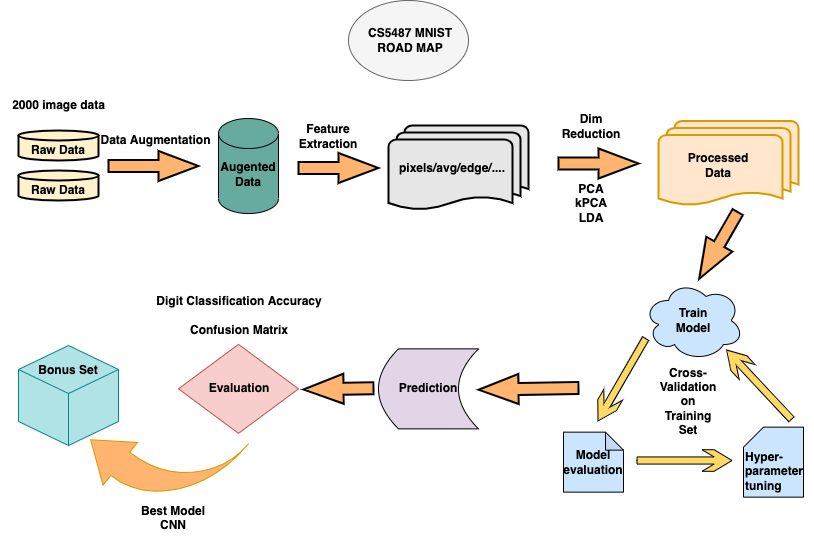
\includegraphics[width=0.95\textwidth]{figure/CS5487.drawio.png}
  \caption{Road Map}
  \label{fig:map}
\end{figure*}
\section{Deep learning Model Demo}
\subsection{MLP} \label{nn}
See Figure~\ref{nn_demo} below.
\begin{figure}[h]
    \centering
    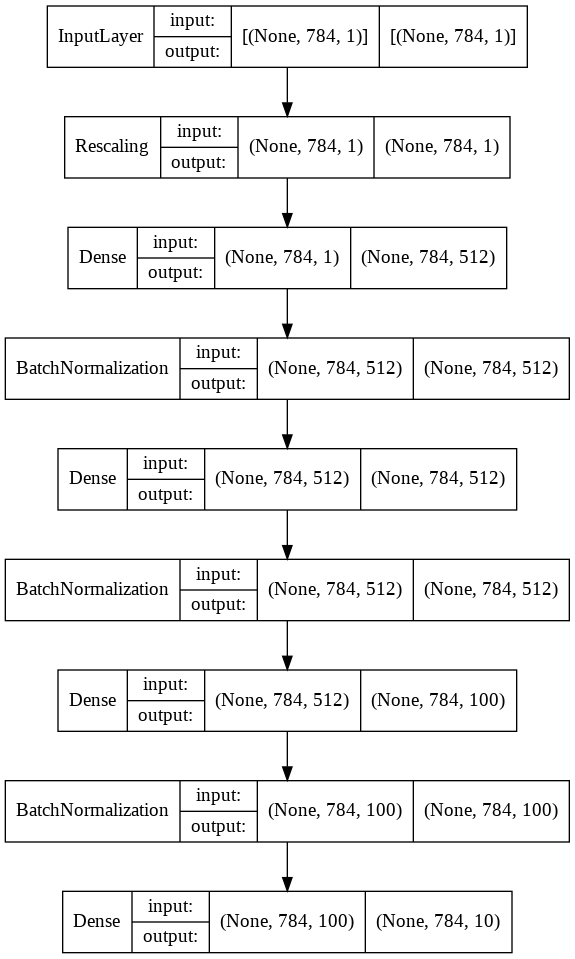
\includegraphics[width=0.49\textwidth]{figure/custom-mlp.png}
    \caption{Multi-Layer Perceptron}
    \label{nn_demo}
\end{figure}
\subsection{CNN-M3} \label{cnn_3}
See Figure~\ref{cnn_m3_demo} below.
\begin{figure}[h]
    \centering
    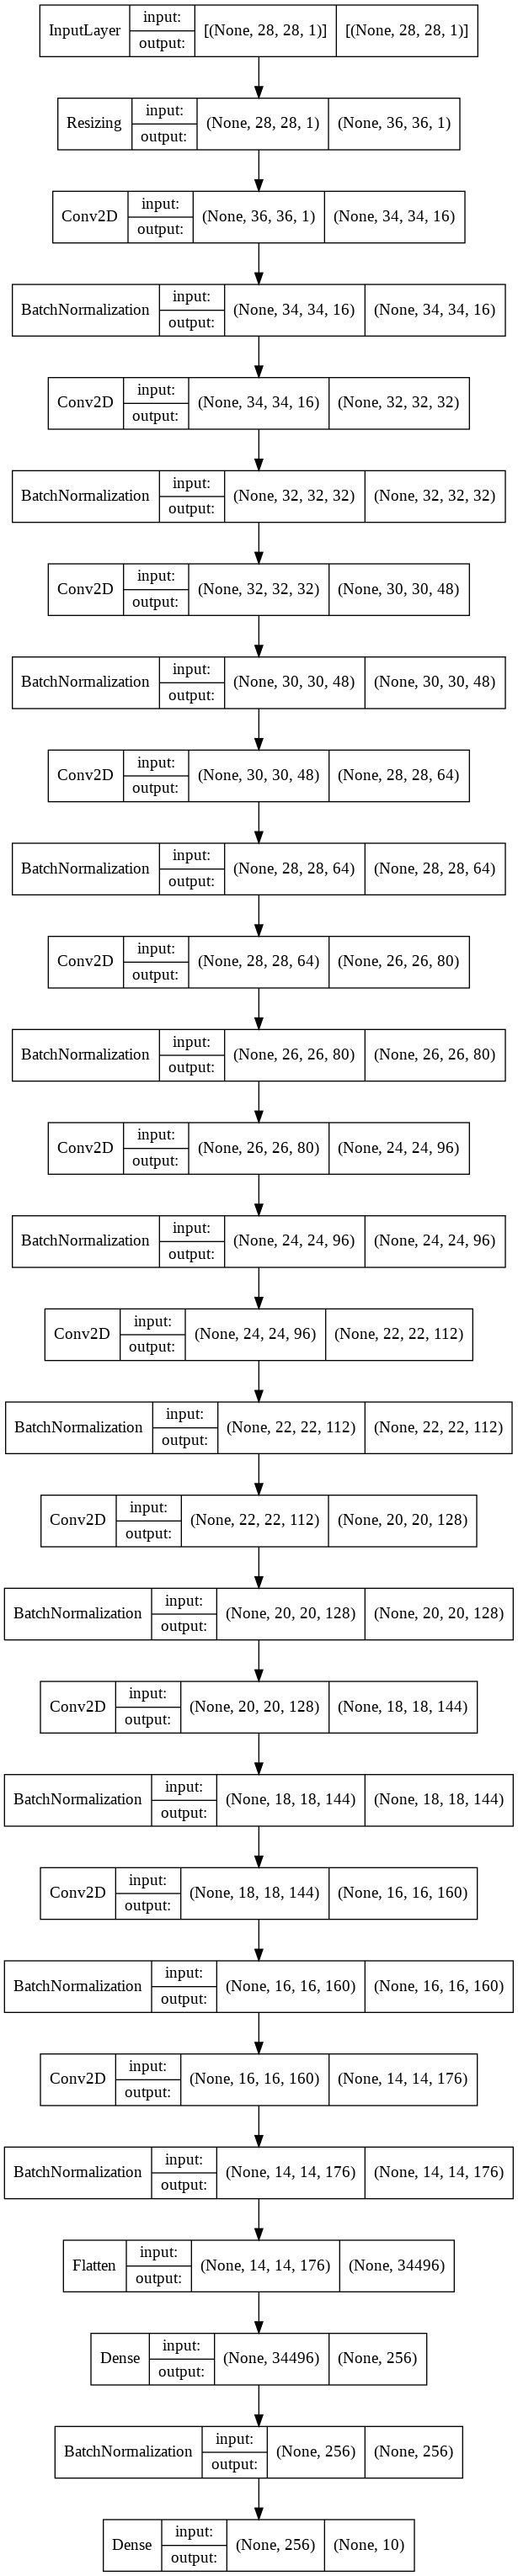
\includegraphics[width=0.25\textwidth]{figure/custom-m3.png}
    \caption{CNN M3}
    \label{cnn_m3_demo}
\end{figure}
\subsection{CNN-M5} \label{cnn_5}
See Figure~\ref{cnn_m5_demo} below.
\begin{figure}[h]
    \centering
    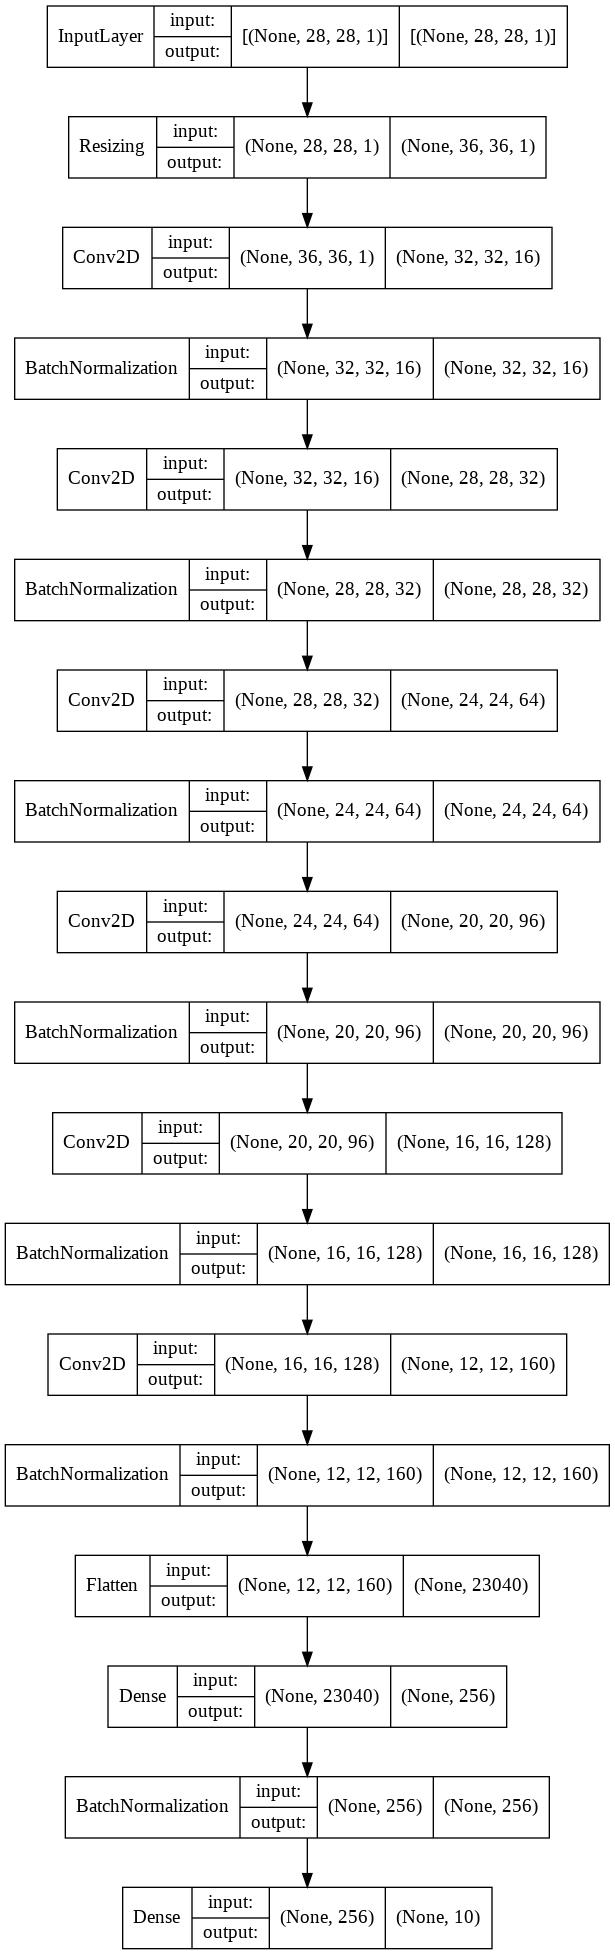
\includegraphics[width=0.40\textwidth]{figure/custom-m5.png}
    \caption{CNN M5}
    \label{cnn_m5_demo}
\end{figure}
\subsection{CNN-M7} \label{cnn_7}
See Figure~\ref{cnn_m7_demo} below.
\begin{figure}[h]
    \centering
    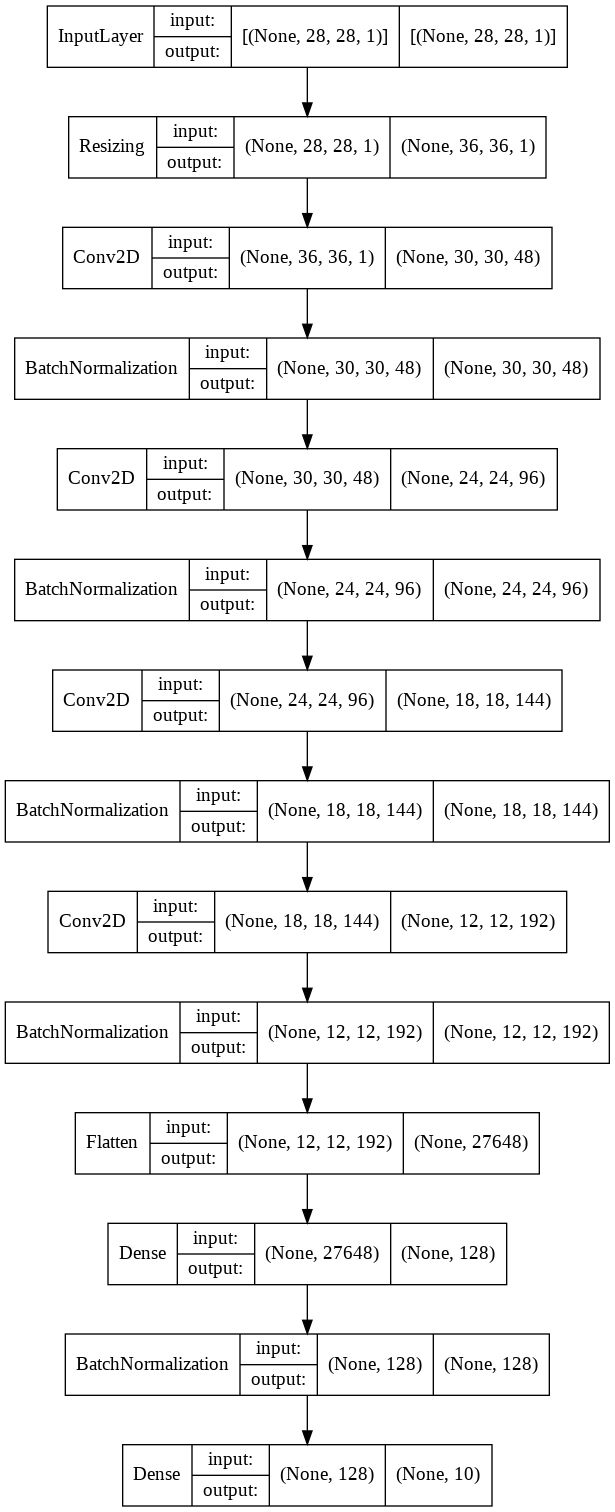
\includegraphics[width=0.49\textwidth]{figure/custom-m7.png}
    \caption{CNN M7}
    \label{cnn_m7_demo}
\end{figure}


\end{document}

